\documentclass[11pt]{report}
\usepackage[utf8]{inputenc}	% Para caracteres en español
\usepackage{amsmath,amsthm,amsfonts,amssymb,amscd}
\usepackage{multirow,booktabs}
\usepackage[table]{xcolor}
\usepackage{fullpage}
\usepackage{lastpage}
\usepackage{enumitem}
\usepackage{fancyhdr}
\usepackage{mathrsfs}
\usepackage{wrapfig}
\usepackage{setspace}
\usepackage{hyperref}
\usepackage{calc}
\usepackage{multicol}
\usepackage{cancel}
\usepackage[retainorgcmds]{IEEEtrantools}
\usepackage[margin=3cm]{geometry}
\usepackage{amsmath}
\newlength{\tabcont}
\setlength{\parindent}{0.0in}
\setlength{\parskip}{0.05in}
\usepackage{empheq}
\usepackage{framed}
\usepackage[most]{tcolorbox}
\usepackage{xcolor}
\colorlet{shadecolor}{orange!15}
\parindent 0in
\parskip 12pt
\geometry{margin=1in, headsep=0.25in}
\theoremstyle{definition}
\usepackage{pdfpages}
\newtheorem{defn}{Definition}
\newtheorem{reg}{Rule}
\newtheorem{exer}{Exercise}
\newtheorem{note}{Note}
\usepackage{fancyhdr}\usepackage{xcolor}\usepackage{amsmath}\usepackage{amssymb}\pagestyle{fancy}\rhead{}
\newtheorem{theorem}{Theorem}[subsection]
\theoremstyle{definition}
\newtheorem{definition}[theorem]{Definiton}
\newtheorem{example}[theorem]{Example}
\newtheorem{corollary}[theorem]{Corollary}
\newtheorem{lemma}[theorem]{Lemma}
\title{Chapter 9 Review Notes}
\begin{document}
\thispagestyle{empty}
{\LARGE \bf ESC 195 Lecture Notes}\\
{\large Hei Shing Cheung}\\
Caculus II, Winter 2024 \hfill ESC 195\\
\\
The up-to-date version of this document can be found at \url{https://github.com/HaysonC/skulenotes}\\

\section{More on Integrals}
\subsection{Riemann Sum - Non-Uniform Petition}
\begin{example}
    Given the following definite integral:
    $$\int^2_0 \sqrt{x} dx$$, we cannot evaluate its Riemann sum with uniforms partition, since the series of root cannot be easily evaluated. 
\end{example}

The definite integral of $\sqrt{x}$ from $0$ to $2$ using a Riemann sum with a non-uniform partition is given by:

$$\int_{0}^{2} \sqrt{x} \, dx = \lim_{n \to \infty} \sum_{i=1}^n \sqrt{x_i} \Delta x_i$$
, where:
\begin{itemize}
    \item $x_0 = 0, \, x_n = 2$,
    \item $x_i = i^2 \cdot \frac{2}{n^2}$ for $i = 0, 1, 2, \dots, n$,
    \item $\Delta x_i = x_i - x_{i-1} = \frac{2}{n^2} \cdot (2i - 1)$.
\end{itemize}

The Riemann sum becomes:
$$
S_n = \sum_{i=1}^n \sqrt{i^2 \cdot \frac{2}{n^2}} \cdot \frac{2}{n^2} \cdot (2i - 1).
$$

Simplifying further:
$$
S_n = \sum_{i=1}^n \sqrt{\frac{2i^2}{n^2}} \cdot \frac{2}{n^2} \cdot (2i - 1).
$$

Taking the limit as $n \to \infty$, the sum converges to the exact value of the integral using the series of squares. 
$$
\int_{0}^{2} \sqrt{x} \, dx = \frac{4\sqrt{2}}{3}.
$$
\paragraph{Condition} $n \to \infty$ Ensures $\Delta x_i \to 0$
\paragraph{} As $n \to \infty$, the partition points $x_i$ become increasingly dense. This ensures that the partition becomes infinitely fine.

\subsection{Integration By Parts}
Using the product rule:
$$
\frac{d}{dx} \big[ u(x) v(x) \big] = u'(x)v(x) + u(x)v'(x),
$$
integrating both sides with respect to $x$ gives:
$$
u(x)v(x) = \int u'(x) v(x) \, dx + \int u(x) v'(x) \, dx.
$$
Rearranging this:
$$\int u'(x) v(x) \, dx = u(x)v(x) - \int u(x) v'(x) \, dx.$$

\paragraph{Integration by parts formula}
\begin{equation}
\int u \, dv = uv - \int v \, du.
\end{equation}
\begin{example}
We want to solve the integral $$ \int x e^{2x} \, dx $$ using integration by parts.

Let:
$$ u = x, \quad dv = e^{2x} \, dx. $$

Then, we compute the derivatives and integrals:
$$ du = dx, \quad v = \frac{e^{2x}}{2}. $$

Now, apply the integration by parts formula:
$$ \int u \, dv = uv - \int v \, du. $$

Substituting in the values:
$$ \int x e^{2x} \, dx = x \cdot \frac{e^{2x}}{2} - \int \frac{e^{2x}}{2} \, dx. $$

Next, compute the remaining integral:
$$ \int \frac{e^{2x}}{2} \, dx = \frac{e^{2x}}{4}. $$

Thus, the result is:
$$ \int x e^{2x} \, dx = \frac{x e^{2x}}{2} - \frac{e^{2x}}{4} + C. $$

\end{example}

\begin{example}
We want to solve $$ \int x^2 \sin(2x) \, dx $$ using double integration by parts.

First, let:
$$ u = x^2, \quad dv = \sin(2x) \, dx. $$

Then:
$$ du = 2x \, dx, \quad v = -\frac{1}{2} \cos(2x). $$

Using the IBP formula:
$$ \int u \, dv = uv - \int v \, du, $$

we get:
$$ \int x^2 \sin(2x) \, dx = -\frac{x^2}{2} \cos(2x) + \int x \cos(2x) \, dx. $$

Now, apply IBP again to \( \int x \cos(2x) \, dx \), let:
$$ u = x, \quad dv = \cos(2x) \, dx. $$

Then:
$$ du = dx, \quad v = \frac{1}{2} \sin(2x). $$

Using the IBP formula again:
$$ \int x \cos(2x) \, dx = \frac{x}{2} \sin(2x) - \int \frac{1}{2} \sin(2x) \, dx, $$

and solving the remaining integral:
$$ \int \frac{1}{2} \sin(2x) \, dx = -\frac{1}{4} \cos(2x). $$

Thus, the final result is:
$$ \int x^2 \sin(2x) \, dx = -\frac{x^2}{2} \cos(2x) + \frac{x}{2} \sin(2x) + \frac{1}{4} \cos(2x) + C. $$

\end{example}
\subsection{Trigonometric Integrals}
\paragraph{Case I} This is the case I trigonometric integrals, the strategy is using the pythagorean identity.
\paragraph{} We want to solve the class of integrals:
\begin{equation}
 \int \sin^n(x) \cos^m(x) \, dx
\end{equation}
, where $m$ or $n$ is odd.
\begin{example}
We want to solve the integral:
$$ I = \int \sin^3(x) \cos^2(x) dx $$
We use the identity: $ \sin^2(x) = 1 - \cos^2(x)$. Thus, the integral becomes:
\begin{align*}
    I &= \int \sin(x)(1 - \cos^2(x)) \cos^2(x) \, dx \\
    &= \int (\cos^2(x) \sin(x) - \cos^4(x) \sin(x)) \, dx
\end{align*} 
which is now easily solvable with substution $u=\cos(x)$.
\end{example}
\paragraph{Case II} The follwoing is generally solvable via case I and case III below. In general, we solve the integral by reducing the power of the trigonometric functions to arrive at a solvable integral Case I or III.
\paragraph{} We want to solve the class of integrals:
\begin{equation} \int \sin^n(x) \cos^m(x) \, dx \end{equation}
, where $m$ and $n$ is even.
\begin{example}
We want to solve the integral:
$$ I = \int \sin^2(x) \cos^4(x) \, dx $$
We can apply the double angle formulas:
\begin{align}
    \sin(x)\cos(x) &= \frac{1}{2} \sin(2x) \\
    \sin^2(x) &= \frac{1 - \cos(2x)}{2} \\
    \cos^2(x) &= \frac{1 + \cos(2x)}{2}
\end{align}
Thus, the integral becomes:
$$ I = \frac{1}{8} \int \sin^2(2x) \, dx + \frac{1}{8} \int \cos(2x)\sin^2(2x) \, dx $$
\end{example}
\paragraph{Case III} This is the case III trigonometric integrals, the strategy is using the reduction formula via IBP.
\paragraph{Reduction Formula} We can solve integrals by reducing the power of the trigonometric functions. These are done using IBP and trigonometric identities.
\paragraph{} We want to solve the classes of integrals:
\begin{equation} 
    \int \sin^n(x) \, dx, \quad \int \cos^n(x) \, dx 
\end{equation}
, where $n$ is a positive integer. For demonstartion, We can obtain the reduction formula of $\sin^n(x)$ via IBP.
\begin{align}
    I_n &= \int \sin^n(x) \, dx \nonumber \\
    &= \int \sin^{n-1}(x) \sin(x) \, dx \nonumber \\
    &= \frac{-\cos(x) \sin^{n-1}(x)}{n} + \frac{(n-1)}{n} \int \cos^2(x) \sin^{n-2}(x) \, dx \nonumber \\
    &= \frac{-\cos(x) \sin^{n-1}(x)}{n} + \frac{(n-1)}{n} I_{n-2}
\end{align}
\paragraph{Reduction for $\cos^n(x)$} We can obtain the reduction formula of $\cos^n(x)$ via IBP.
\begin{align}
    I_n &= \int \cos^n(x) \, dx \nonumber \\
    &= \int \cos^{n-1}(x) \cos(x) \, dx \nonumber \\
    &= \frac{\sin(x) \cos^{n-1}(x)}{n} + \frac{(n-1)}{n} \int \sin^2(x) \cos^{n-2}(x) \, dx \nonumber \\
    &= \frac{\sin(x) \cos^{n-1}(x)}{n} + \frac{(n-1)}{n} I_{n-2}
\end{align} 
\paragraph{Case IV} The following is generally solvable via simple trigonometric integrals. In general, we solve the integral by applying the angle sum formulas.
\paragraph{} We want to solve the classes of integrals:
\begin{equation}
    \int \sin(mx) \cos(nx) \, dx, \quad \int \sin(mx) \sin(nx) \, dx, \quad \int \cos(mx) \cos(nx) \, dx 
\end{equation}
We could apply the angle sum formulas:
\begin{align}
    \sin(mx)\cos(nx) &= \frac{1}{2} \left[ \sin((m+n)x) + \sin((m-n)x) \right] \\
    \sin(mx)\sin(nx) &= \frac{1}{2} \left[ \cos((m-n)x) - \cos((m+n)x) \right] \\
    \cos(mx)\cos(nx) &= \frac{1}{2} \left[ \cos((m-n)x) + \cos((m+n)x) \right]
\end{align}
\paragraph{Case V} The following is generally solvable via the following trigonometric identities listed below, which convert it into a reduction formula.
\begin{align}
    \tan^2(x) &= \sec^2(x) - 1 \label{eq:tan2} \\
    \cot^2(x) &= \csc^2(x) - 1 \label{eq:cot2}  \\
    \frac{d}{dx} \tan(x) &= \sec^2(x)
\end{align}
\paragraph{} We want to solve the classes of integral:
\begin{equation}
    \int \tan^n(x) \, dx, \quad \int \cot^n(x) \, dx 
\end{equation}
We know that $tan^2(x) = \sec^2(x) - 1$. Thus, we can solve the integral by reducing the power of the tangent function.
\paragraph{Reduction for $\tan^n(x)$} We can obtain the reduction formula of $\tan^n(x)$ via the trigonometric identities.
\begin{align}
    I_n &= \int \tan^n(x) \, dx \nonumber \\
    &= \int \tan^{n-1}(x) \tan(x) \, dx \nonumber \\
    &= \frac{\tan^{n-1}(x)}{n-1} - \int \tan^{n-2}(x) \, dx \nonumber \\
    &= \frac{\tan^{n-1}(x)}{n-1} - I_{n-2}
\end{align}
\paragraph{Reduction for $\cot^n(x)$} We can obtain the reduction formula of $\cot^n(x)$ via the trigonometric identities.
\begin{align}
    I_n &= \int \cot^n(x) \, dx \nonumber \\
    &= \int \cot^{n-1}(x) \cot(x) \, dx \nonumber \\
    &= \frac{\cot^{n-1}(x)}{n-1} - \int \cot^{n-2}(x) \, dx \nonumber \\
    &= \frac{\cot^{n-1}(x)}{n-1} - I_{n-2}
\end{align}
\paragraph{Case VI} The following is generally solvable via the trigonometric identities (\ref{eq:tan2}) and (\ref{eq:cot2}).
\paragraph{} We want to solve the classes of integral:
\begin{equation} 
    \int \tan^m(x) \sec^n(x) \, dx, \quad \int \cot^m(x) \csc^n(x) \, dx 
\end{equation}
We can solve the integral by reducing the power of the converted trigonometric functions using (\ref{eq:tan2}) and (\ref{eq:cot2}).
\paragraph{Case VII} The following is generally solvable via the trigonometric identities (\ref{eq:tan2}) and (\ref{eq:cot2}).
\paragraph{} We want to solve the classes of integral:
\begin{equation} \int \tan^m(x) \sec^n(x) \, dx, \quad \int \cot^m(x) \csc^n(x) \, dx \end{equation}
We can solve the integral by converting between the tangent and secant functions using the trigonometric identities.
\paragraph{Case VIII} This is the case VIII integrals, the strategy is using the trigonometric substitution.
\paragraph{Trigonometric Substitution} We can solve integrals by substituting the trigonometric functions with other trigonometric functions.
\begin{example}
We want to solve the integral:
$$ \int \frac{dx}{\sqrt{1 - x^2}} $$
\end{example}
We can substitute $x = \sin(\theta)$, then $dx = \cos(\theta) \, d\theta$. The integral becomes:
$$ \int \frac{\cos(\theta) \, d\theta}{\sqrt{1 - \sin^2(\theta)}} = \int \frac{\cos(\theta) \, d\theta}{\cos(\theta)} = \int d\theta = \theta + C. $$
\paragraph{} In general, we can use the following substitutions:
\begin{itemize}
    \item $x = a\sin(\theta)$ for $\sqrt{a^2 - x^2}$,
    \item $x = a\tan(\theta)$ for $\sqrt{a^2 + x^2}$,
    \item $x = a\sec(\theta)$ for $\sqrt{x^2 - a^2}$.
\end{itemize}
\paragraph{Weierstrass Substitution} We can solve integrals by using the Weierstrass substitution:
\begin{equation}
    \tan\left(\frac{x}{2}\right) = t \Leftrightarrow \cos(x) = \frac{1-t^2}{1+t^2} \quad \sin(x) = \frac{2t}{1+t^2} \quad dx = \frac{2dt}{1+t^2}
\end{equation}
This substitution is useful for solving integrals with trigonometric functions, by converting them into rational functions.
\paragraph{Summary} We can solve trigonometric integrals by using the following strategies:
\begin{table}[h!]
    \centering
    \begin{tabular}{|c|l|}
    \hline
    \textbf{Case} & \textbf{Strategy and General Form} \\ \hline
    I   & Use \(\sin^2(x) + \cos^2(x) = 1\); simplify using substitution. \\
        & General Form: \(\int \sin^n(x) \cos^m(x) dx\), where \(m\) or \(n\) is odd. \\ \hline
    II  & Convert to Case I and Case III using double angle formulas. \\
        & General Form: \(\int \sin^n(x) \cos^m(x) dx\), where both \(m\) and \(n\) are even. \\ \hline
    III & Apply reduction formulas derived via integration by parts. \\
        & General Form: \(\int \sin^n(x) dx\) or \(\int \cos^n(x) dx\). \\ \hline
    IV  & Use angle sum formulas to simplify. \\
        & General Form: \(\int \sin(mx) \cos(nx) dx\). \\ \hline
    V   & Reduce tangent/cotangent powers using \(\tan^2(x) = \sec^2(x) - 1\) and substitution. \\
        & General Form: \(\int \tan^n(x) dx\) or \(\int \cot^n(x) dx\). \\ \hline
    VI  & Convert to Case V via Pythagorean identities. \\
        & General Form: \(\int \tan^m(x) \sec^n(x) dx\) or \(\int \cot^m(x) \csc^n(x) dx\). \\ \hline
    VII & Convert between tangent and secant functions for simplification. \\
        & General Form: \(\int \tan^m(x) \sec^n(x) dx\). \\ \hline
    VIII & Use trigonometric substitution: \(x = a \sin(\theta), a \tan(\theta), a \sec(\theta)\). \\
         & General Form: \(\int \frac{dx}{\sqrt{a^2 - x^2}}, \int \frac{dx}{\sqrt{a^2 + x^2}}, \int \frac{dx}{\sqrt{x^2 - a^2}}\). \\ \hline
    \end{tabular}
    \caption{Strategies and General Forms for Case I-VIII Integrals}
\end{table}
\subsection{Partial Fractions}
\paragraph{Partial Fraction Decomposition} We can decompose a rational function into partial fractions to simplify integration.
\paragraph{} We want to solve the integral:
\begin{equation}
    \int \frac{P(x)}{Q(x)} \, dx
\end{equation}
, where $P(x)$ and $Q(x)$ are polynomials.
\begin{example}
We want to solve the integral:
$$ \int \frac{2x^2 + 3x + 1}{x^3 + 2x^2 + x} \, dx $$
\end{example}
We can decompose the rational function into partial fractions:
$$ \frac{2x^2 + 3x + 1}{x^3 + 2x^2 + x} = \frac{A}{x} + \frac{B}{x+1} + \frac{C}{(x+1)^2} $$
\paragraph{} We can solve for the constants $A$, $B$, and $C$ by equating the coefficients of the partial fractions to the original function. We have:
\begin{align*}
    2x^2 + 3x + 1 &= A(x+1)^2 + Bx(x+1) + Cx \\
    \intertext{Thus, we can solve it by setting $x = 0$, $x = -1$}
\end{align*}
\paragraph{Summary} We can solve integrals using partial fraction decomposition by following these steps:
\begin{table}[h!]
    \centering
    \begin{tabular}{|c|l|}
    \hline
    \textbf{Step} & \textbf{Description} \\ \hline
    1 & Factorize the denominator of the rational function. \\
    2 & Write the partial fraction decomposition. \\
    3 & Solve for the constants by equating the coefficients. \\
    4 & Integrate the partial fractions. \\ \hline
    \end{tabular}
    \caption{Steps for Partial Fraction Decomposition}
\end{table}
\subsection{Improper Integrals}
\paragraph{Improper Integral} An improper integral is an integral with an infinite limit or a discontinuity in the interval of integration.
\paragraph{} We want to solve the integral:
\begin{equation}
    \int_a^b f(x) \, dx
\end{equation}
, where $a$ or $b$ is infinite or $f(x)$ is discontinuous.
\begin{example}
We want to solve the integral:
$$ \int_0^\infty e^{-x} \, dx $$

Evaluating the integral:
\begin{align*}
    \int_0^\infty e^{-x} \, dx &= \lim_{b \to \infty} \int_0^b e^{-x} \, dx \\
    &= \lim_{b \to \infty} -e^{-x} \Big|_0^b \\
    &= \lim_{b \to \infty} -e^{-b} + 1 \\
    &= 1
\end{align*}
\end{example}
\subsection{Convergence Test}
\paragraph{Convergence} An improper integral converges if the limit of the integral exists. 
\paragraph{Comparison Test} We can compare the integral to another integral to determine convergence or divergence.
\paragraph{Spliting the Integral} We can split the integral into two parts to determine convergence. We split it into two limits on the left and right, for example:
$$ \int_a^b f(x)\, dx = \lim_{t \to c^-} \int_a^t f(x) \, dx + \lim_{t \to c^+} \int_t^b f(x) \, dx $$
\section{Hyperbolic Trigonometric Functions}
\begin{definition}[Hyperbolic Sine]
    The hyperbolic sine function is defined as:
    \begin{equation} \sinh(x) = \frac{e^x - e^{-x}}{2}. \end{equation}
\end{definition}
\begin{definition}[Hyperbolic Cosine]
    The hyperbolic cosine function is defined as:
    \begin{equation}  \cosh(x) = \frac{e^x + e^{-x}}{2}. \end{equation}
\end{definition}
\paragraph{Properties} These combinations of exponential functions have properties similar to the trigonometric functions.
\paragraph{Derivatives} The derivatives of the hyperbolic functions are:
\begin{align}
    \frac{d}{dx} \sinh(x) &= \cosh(x), \\
    \frac{d}{dx} \cosh(x) &= \sinh(x).
\end{align}
\paragraph{Identities} The hyperbolic functions satisfy the following identities:
\begin{align}
    \cosh^2(x) - \sinh^2(x) &= 1, \\
    \cosh(2x) &= \cosh^2(x) + \sinh^2(x), \\
    \sinh(2x) &= 2\sinh(x)\cosh(x).
\end{align}
\paragraph{Hyperbola} The hyperbolic functions are related to the hyperbola $x^2 - y^2 = 1$. Simiar to the circle, the hyperbola can be parametrized by the hyperbolic functions (e.g. $x = \cosh(t)$, $y = \sinh(t)$).
\paragraph{Area} The area of a sector of the hyperbola is given by:
\begin{equation}
    A = t/2,
\end{equation} 
where $t$ is the angle of the sector along the parametrization $\{(x,y)\mid x = \cosh(t), y = \sinh(t)\}$.
\begin{figure}[h!]
    \begin{center}
        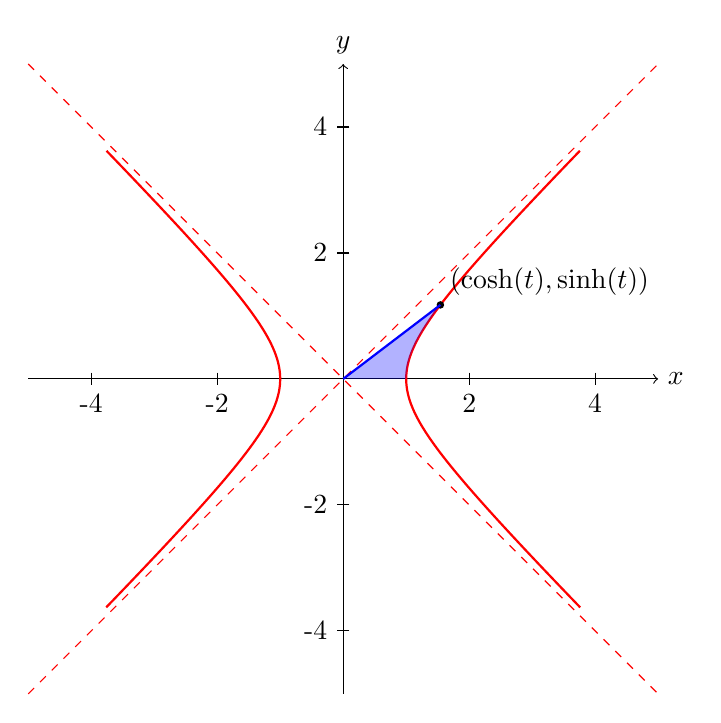
\begin{tikzpicture}[scale=0.8]
            % Draw the axes
            \draw[->] (-5, 0) -- (5, 0) node[right] {$x$};
            \draw[->] (0, -5) -- (0, 5) node[above] {$y$};
        
            % Draw ticks on the axes
            \foreach \x in {-4, -2, 2, 4}
                \draw (\x, 0.1) -- (\x, -0.1) node[below] {\x};
            \foreach \y in {-4, -2, 2, 4}
                \draw (0.1, \y) -- (-0.1, \y) node[left] {\y};
        
            % Draw the hyperbola branches
            \draw[thick, red, domain=-2:2, samples=100] plot ({cosh(\x)}, {sinh(\x)});
            \draw[thick, red, domain=-2:2, samples=100] plot ({-cosh(\x)}, {sinh(\x)});
        
            % Draw the asymptotes
            \draw[red, dashed] (-5, -5) -- (5, 5);
            \draw[red, dashed] (-5, 5) -- (5, -5);
        
            % Add a point on the hyperbola
            \coordinate (P) at ({cosh(1)}, {sinh(1)});
            \draw[fill] (P) circle (0.05) node[above right] {$(\cosh(t), \sinh(t))$};
        
            % Connect the labeled point to the origin
            \draw[thick, blue] (0, 0) -- (P);
        
            % Fill the sector area between hyperbola, line, and x-axis
            \fill[blue, opacity=0.3, domain=0:1, variable=\t]
                (0, 0) -- plot ({cosh(\t)}, {sinh(\t)}) -- cycle;
        \end{tikzpicture}
    \end{center}
    \caption{Sector of the hyperbola}
    \centering
\end{figure}
\paragraph{Catenary} The hyperbolic cosine function describes the shape of a hanging chain or cable. The catenary is the curve formed by a chain hanging from two points. It is given by the equation:
\begin{equation}
    a \cosh\left(\frac{x}{a}\right),
\end{equation}
\begin{definition}[Hyperbolic Tangent]
    The hyperbolic tangent function is defined as:
    \begin{equation}
        \tanh(x) = \frac{\sinh(x)}{\cosh(x)} = \frac{e^x - e^{-x}}{e^x + e^{-x}}. 
    \end{equation}
\end{definition}
\paragraph{Derivative} The derivative of the hyperbolic tangent function resembles the derivative of the regular tangent function:
\begin{equation} \frac{d}{dx} \tanh(x) = \text{sech}^2(x). \end{equation}
\paragraph{Identities} The hyperbolic tangent function satisfies the following identities:
\begin{align}
    \tanh(x) &= \frac{\sinh(x)}{\cosh(x)}, \\
    \text{sech}^2(x) &= 1 - \tanh^2(x).
\end{align}
\paragraph{Secant, Cosecant, Cotangent} The hyperbolic secant, cosecant, and cotangent functions are defined similarly to the regular secant, cosecant, and cotangent functions. They are the \textbf{reciprocal} of the hyperbolic cosine, sine, and tangent functions, respectively.
\paragraph{Inverse Hyperbolic Functions} The inverse hyperbolic functions are defined as the inverse of the hyperbolic functions. They are denoted by $\sinh^{-1}(x)$, $\cosh^{-1}(x)$, $\tanh^{-1}(x)$, etc.
\begin{align}
    \text{arsinh } x &= \ln\left(x + \sqrt{x^2 + 1}\right) \\[10pt]
    \text{arcosh } x &= \ln\left(x + \sqrt{x^2 - 1}\right) \\[10pt]
    \text{artanh } x &= \frac{1}{2} \ln\left(\frac{1 + x}{1 - x}\right) \\[10pt]
    \text{arcsch } x &= \ln\left(\frac{1}{x} + \sqrt{\frac{1}{x^2} + 1}\right) \\[10pt]
    \text{arsech } x &= \ln\left(\frac{1}{x} + \sqrt{\frac{1}{x^2} - 1}\right) \\[10pt]
    \text{arcoth } x &= \frac{1}{2} \ln\left(\frac{x + 1}{x - 1}\right)
\end{align}
\section{Further Applications of Integrals}
\subsection{Arc Length}
\paragraph{Arc Length}
    Given the curve $C: y = f(x)$, the arc length of the curve between two points $a$ and $b$, where $y'(x)$ is continuous, we would like the compute the arc length of the curve:
    $$ L = \int_C ds$$
\paragraph{Formula} We can derive the formula for the arc length of a curve $y = f(x)$ between two points $a$ and $b$ as:
\begin{align}
    \intertext{At $x_i$ and $x_{i+1}$, the length of the segment is:}
    \Delta s &\approx \sqrt{(x_{i+1} - x_i)^2 + (y_{i+1} - y_i)^2} \nonumber \\
            &= \sqrt{\Delta_i x^2 + \Delta_i y^2} \nonumber \\
    \intertext{We also have, by MVT:}
    \frac{\Delta y}{\Delta x} &= y'(c) \nonumber \\
    \Delta y &= y'(c) \Delta x \nonumber \\
    \Delta s &\approx \sqrt{\Delta x^2 + (y'(c) \Delta x)^2} \nonumber \\
            &= \sqrt{1 + y'(c)^2} \Delta x \nonumber \\
    \intertext{Taking a Riemann sum:}
    L &= \lim_{n \to \infty} \sum_{i=1}^n \sqrt{1 + y'(c_i)^2} \Delta x \nonumber \\
    &= \int_a^b \sqrt{1 + y'(x)^2} \, dx 
\end{align}
\begin{example}
    Given $f(x) = x^\frac{3}{2}$ between $x = 0$ and $x = 44$, we would like to compute the arc length of the curve:
    \begin{align*}
        L &= \int_0^{44} \sqrt{1 + \left(\frac{3}{2}x^{\frac{1}{2}}\right)^2} \, dx \\
        &= \int_0^{44} \sqrt{1 + \frac{9}{4}x} \, dx \\
        &= \frac{8}{27} \left(1 + \frac{9}{4}x\right)^{\frac{3}{2}} \Big|_0^{44} = 296
    \end{align*}
\end{example}
\paragraph{Inverse} Also, we can take $x = f^{-1}(y)$ to compute the arc length of a curve.
\begin{equation}
    L = \int_{f(a)}^{f(b)} \sqrt{1 + ((f{^{-1}})'(y))^2} \, dy
\end{equation}
\subsection{Surface Area of Revolution}
\paragraph{Surface Area of Revolution} Given the curve $C: y = f(x)$, we would like to compute the surface area of the curve between two points $a$ and $b$ when rotated about the $x$-axis:
    $$ A_x = \int_C 2\pi y \, ds$$
\paragraph{Formula} Deriving the formula for the surface area of a curve $y = f(x)$ between two points $a$ and $b$ rotated about the $x$-axis as follows:
\begin{align}
    \intertext{At $x_i$ and $x_{i+1}$, the length of the segment is:}
    \Delta s &\approx \sqrt{\Delta_i x^2 + \Delta_i y^2} \nonumber \\
    \intertext{The surface area of the segment is, by continuity:}
    A_i &= \pi (y_i + y_{i+1}) \Delta s = 2\pi y^\star \Delta s \quad 
    \intertext{As the difference between $y^\star$ and $y_i$ diminishes as $\Delta x \rightarrow 0$, taking a Riemann sum:}
    A_x &= \lim_{n \to \infty} \sum_{i=1}^n 2\pi y_i \sqrt{\Delta_i x^2 + \Delta_i y^2} \nonumber \\
    &= \int_a^b 2\pi y \sqrt{1 + y'(x)^2} \, dx
    \intertext{The surface area of a curve $y = f(x)$ (i.e. $x = f^{-1}$)between two points $f(a)$ and $f(b)$ rotated about the $y$-axis is:}
    A_y &= \int_{f(a)}^{f(b)} 2\pi x \sqrt{1 + x'(y)^2} \, dy
\end{align}
\begin{example}
    Given $y = \sqrt{x}$ between $x = 0$ and $x = 1$, we would like to compute the surface area of the curve:
    \begin{align*}
        A_x &= \int_0^1 2\pi \sqrt{x} \sqrt{1 + \frac{1}{4x}} \, dx \\
        &= \pi \int^1_0 \sqrt{4x + 1} \, dx \\
        \intertext{Let $u = 4x + 1$, then $du = 4dx$:}
        &= \frac{\pi}{4} \int^5_1 \sqrt{u} \, du \\
        &= \frac{\pi}{6}\left(5^\frac{3}{2} -1\right)
    \end{align*}
\end{example}
\subsection{Applications to Physics and Engineering}
\subsubsection{Hydrostatic Pressure and Force}
\paragraph{Hydrostatic Pressure} The hydrostatic pressure and Force is given by the Archimedes' principle:
\begin{subequations}
    \begin{align}
        P &= \rho g \cdot d, \\
        F &= \rho g \cdot d \cdot A
    \end{align}
\end{subequations}
\paragraph{Riemann Sum} Given a tank rectangular with width defined by $w = f(x)$, we can take a horizontal slice, $x^\star$, of the tank to compute the force exerted on the tank by the water:
\begin{equation}
    F =\sum_{i=1}^n \rho g x_i f(x_i) \Delta x
\end{equation}
\paragraph{Formula} Given a tank rectangular with width defined by $w = f(x)$, where $x$ is depth, we would like to compute the force exerted on the tank by the water:
\begin{equation}
    F = \int_0^b \rho g x f(x) \cdot dx
\end{equation}
, which is derived by considering $dx$ as the depth a horizontal slice of the tank.
\subsubsection{Center of Mass and Moments of Inertia}
\paragraph{Properties of the Center of Mass} The center of mass of a region $R$ has the following properties:
\begin{enumerate}
    \item \textbf{Symetry}: For all axis of symmetry, the center of mass lies on the axis.
    \item \textbf{Additivity}: The center of mass of a region is the weighted average of the centers of mass of its parts. The weights are the areas of the parts.
    \begin{equation}
        \bar{x} = \sum_i \frac{A_i\bar{x_i}}{A}
    \end{equation}
\end{enumerate}
\paragraph{Formula} The centroid of a uniformly-dense region $R$ bounded by $y=f(x),\,x\in[a,b],\,y\in[f(a),f(b)]$ is derived as follows:
\begin{align}
    \intertext{We first have $x_i^\star$ and $A_i$ as follows:}
    x_i^\star = \frac{1}{2}(x_i + x_{i+1}) &\quad A_i = f(x_i) \Delta x \nonumber \\
    \intertext{For $\bar{x}$, we have:}
    A\bar{x} &\approx \sum_i x_i^\star A_i \nonumber \\
    \intertext{Taking a Riemann sum:}
    A\bar{x} &= \lim_{n \to \infty} \sum_i x_i^\star A_i  \nonumber \\
    \bar{x} &= \frac{1}{A}\int_a^b x f(x) \, dx
    \intertext{Similarly, for $\bar{y}$:}
    A\bar{y} &= \lim_{n \to \infty} \sum_i f(x_i^\star) A_i \nonumber \\
    \bar{y} &= \frac{1}{A}\int_a^b \frac{1}{2}(f(x))^2 \, dx
\end{align}
\begin{theorem}[Pappus's Theorem]
    The volume of a solid of revolution is given by the product of the area of the region and the distance, $R$, traveled by the centroid of the region from the axis of rotation.
    \begin{equation}
        V = 2\pi R A
    \end{equation}
\end{theorem}
\begin{example}[Eliptical Torus]
    Given an eliptical torus (tall donut) with major axis $a$ and minor axis $b$, we would like to compute the volume of the torus:
    \begin{align*}
        V &= 2\pi R A \\
        &= 2\pi R \cdot \pi ab = 2\pi^2 abR
    \end{align*}
    This could be, alternatively, shown via the washer method and the shell method.
\end{example}
\subsection{Applications to Economics and Biology}
``Biologists are so bad at math'' - Prof. Davis as he proceeds to erase the board and skip to the next section.
\section{Parametric Equations and Polar Coordinates}
\subsection{Curves Defined by Parametric Equations}
\paragraph{Parametric Equations} For $t \in \mathbb{R}$, we have:
\begin{equation}
    x = x(t), \quad y = y(t)
\end{equation}
\begin{example}[Newton's Laws of Motion]
    Given $\ddot{x} = 0$, $\ddot{y} = -g$, we have:
    \begin{align*}
        x(t) &= A_1 t + A_2, \\
        y(t) &= -\frac{1}{2}gt^2 + B_1 t + B_2
    \end{align*}
    At initial conditions $t = 0$, we have $x(0) = 0$, $y(0) = 0$, $\dot x(0) = v_0 \cos(\theta)$, $\dot y(0) = v_0 \sin(\theta) - \frac{1}{2}gt^2$.
\end{example}
\begin{example}[Ellipse]
    Given $x = a\cos(t)$, $y = b\sin(t)$, we have:
    \begin{align*}
        x^2 &= a^2\cos^2(t), \\
        y^2 &= b^2\sin^2(t)
    \end{align*}
    , which satisfies $x^2/a^2 + y^2/b^2 = 1$.
\end{example}
\paragraph{Intersections of Parametric Curves} Given two parametric curves $C_1,\,C_2$, defined by:
\begin{align*}
    C_1:\, x_1 &= x_1(t), \quad y_1 = y_1(t) \\
    C_2:\, x_2 &= x_2(t), \quad y_2 = y_2(t)
\end{align*}
, we can find the intersection points by solving the system of equations:
\begin{align*}
    x_1(t) &= x_2(t) \\
    y_1(t) &= y_2(t)
\end{align*}
\begin{example}
    Given $x_1 = 2t+t$, $y_1 = 5-4t$, $x_2 = 3 - 5\cos(\pi t)$, $y_2 = 1 + 5\sin(\pi t)$, we have:
    \begin{align*}
        2t + 1 &= 3 - 5\cos(\pi t) \\
        5 - 4t &= 1 + 5\sin(\pi t)
    \end{align*}
\end{example}
\subsection{Calculus with Parametric Curves}
\paragraph{Tangents} The tangent to a parametric curve $C$ at a point $t$ is given by:
\begin{equation}
    \frac{dy}{dx} = \frac{dy/dt}{dx/dt} = \frac{y'(t)}{x'(t)}
\end{equation}
\paragraph{Equation of the Tangent} The equation of the tangent to a parametric curve $C$ at a point $t_0$ is given by:
\begin{equation}
    y'(t_0) (x-x(t_0)) - x'(t_0) (y-y(t_0)) = 0
\end{equation}
Hence, if $x'(t_0) = 0$, we have a vertical tangent; if $y'(t_0) = 0$, we have a horizontal tangent. However, if $x'(t_0) = 0$ and $y'(t_0) = 0$, we have no information.
\begin{example}
    Let $x = \sin 2t$, $y = \sin t$, we have:
    \begin{align*}
        x'(t) &= 2\cos 2t, \\
        y'(t) &= \cos t
    \end{align*}
    \textbf{Vertical Tangent}: $2\cos 2t = 0 \Rightarrow t = \frac{\pi}{4} + \frac{n\pi}{2}$.
    \textbf{Horizontal Tangent}: $\cos t = 0 \Rightarrow t = \frac{\pi}{2} + n\pi$.
    \textbf{At $t = 0$} we have $x' = y' = 0$. Thus, we have no information. On the graph, we see that the curve intersects itself at $t = 0$.
\end{example}
\paragraph{Area under Parametric Curve} The area under a parametric curve $C$ between $t_1$ and $t_2$ is given by:
\begin{equation}
    A = \int^{x(t_2)}_{x(t_1)} y(x) \, dx = \int_{t_1}^{t_2} y(t) x'(t) \, dt 
\end{equation}
\begin{definition}[Orientation]
    The orientation of a parametric curve $C$ is given by the direction of the curve as $t$ increases. If the enclosed area is to the left of the trace of $t$ (counter-clockwise) the orientation is positive; otherwise, it is negative.
\end{definition}
\paragraph{} The sign of the area of a parametric curve $C$ is given by the orientation of the curve.
\paragraph{Area of Closed Curves} The area of a closed parametric curve $C$ is given by:
\begin{equation}
    A = \oint_C dA = \int_{t_1}^{t_2} y(t) x'(t) \, dt = \int_{t_1}^{t_2} x(t) y'(t) \, dt
\end{equation}
, where
\begin{equation*}
    x(t_1) = x(t_2), \quad y(t_1) = y(t_2) \quad \text{and} \quad \text{$t_2$ is the smallest $t>t_1$ to satisfy the condition}.
\end{equation*}
\paragraph{Arc Length} The arc length of a parametric curve $C$ is given by:
\begin{equation}
    L = \int_a^b \sqrt{\left(\frac{dx}{dt}\right)^2 + \left(\frac{dy}{dt}\right)^2} \, dt
\end{equation}
\begin{example}
    Given $x = t\cos t$, $y = t\sin t$, we have:
    \begin{align*}
        \frac{dx}{dt} &= \cos t - t\sin t, \\
        \frac{dy}{dt} &= \sin t + t\cos t
    \end{align*}
    Thus, the arc length is given by:
    \begin{align*}
        L &= \int_0^{2\pi} \sqrt{(\cos t - t\sin t)^2 + (\sin t + t\cos t)^2} \, dt \\
        &= \int_0^{2\pi} \sqrt{1 + t^2} \, dt
        \intertext{Using the substitution $t = \tan \theta$, we have:}
        &= \pi \sqrt{1 + 4\pi^2} + \frac{1}{2}\ln(2\pi + \sqrt{1 + 4\pi^2})
    \end{align*}
\end{example}
\paragraph{Surface Area of Revolution} The surface area of a parametric curve $C$ rotated about the $x$-axis is given by:
\begin{align}
    A &= \int_a^b 2\pi y(t) ds \nonumber \\
    \intertext{From the arc length formula, we have $ds = \sqrt{(\frac{dx}{dt})^2 + (\frac{dy}{dt})^2} \, dt$, thus:}
    &= \int_a^b 2\pi y(t) \sqrt{\left(\frac{dx}{dt}\right)^2 + \left(\frac{dy}{dt}\right)^2} \, dt
\end{align}
Similarly, the surface area of a parametric curve $C$ rotated about the $y$-axis is given by:
\begin{equation}
    A = \int_a^b 2\pi x(t) \sqrt{\left(\frac{dx}{dt}\right)^2 + \left(\frac{dy}{dt}\right)^2} \, dt
\end{equation}
\begin{example}[Surface Area of of a Ellipse]
    Given $x = a\sin t$, $y = b\cos t$, we have:
    \begin{align*}
        \frac{dx}{dt} &= a\cos t, \\
        \frac{dy}{dt} &= -b\sin t
    \end{align*}
    Thus, the surface area of the ellipse is given by:
    \begin{align*}
        A &= \int_0^{2\pi} 2\pi b\cos t \sqrt{a^2\cos^2 t + b^2\sin^2 t} \, dt \\
        &= 2\pi b \int_0^{2\pi} \sqrt{a^2 (1 - \sin^2 t) + b^2 \sin^2 t} \, dt \\
        &= 2\pi b \int_0^{2\pi} \sqrt{a^2 + b^2 - (a^2 - b^2)\sin^2 t} \, dt
    \end{align*}
    This has no analytical solution, but can be solved numerically. Typically, we take $\epsilon = \sqrt{\frac{a^2-b^2}{a^2}}$.
\end{example}
\section{Polar Coordinates}
\paragraph{Polar Coordinates} Given a point $P$ in the plane, we can define the polar coordinates of $P$ as $(r, \theta)$, where $r$ is the distance from the origin to $P$ and $\theta$ is the angle between the positive $x$-axis and the line segment from the origin to $P$.
\paragraph{Transformation} We can convert between polar and Cartesian coordinates as follows:
\begin{equation}
    x = r\cos \theta, \quad y = r\sin \theta
\end{equation}
\paragraph{Reverse Transformation} We can convert between Cartesian and polar coordinates as follows:
\begin{equation}
    r = \sqrt{x^2 + y^2}, \quad \theta = \arctan\left(\frac{y}{x}\right)
\end{equation}
\paragraph{Note} The angle $\theta$ is not unique, as $\theta + 2\pi n$ for $n \in \mathbb{Z}$ represents the same point, beware of this when converting between polar and Cartesian coordinates.
\begin{example}[Lines]
    \begin{align*}
        y = mx + b &\implies \theta = \alpha = \arctan m \\
        x = a &\implies r = a\sec \theta \\
        y = a &\implies r = a\csc \theta
    \end{align*}
\end{example}
\begin{example}[Cirlces]
    \begin{align*}
        x^2 + y^2 = a^2 &\implies r = a \\
    \end{align*}
    Let $r = 6\sin \theta$, we have:
    \begin{align*}
        r^2 &= 6r\sin \theta \\
        x^2 + y^2 &= 6y \\
        x^2 + (y-3)^2 &= 9
    \end{align*}
    We deduce that the curve is a circle with radius $3$ and center $(0,3)$.
\end{example}
\paragraph{Cylinrical Coordinates} Given a point $P$ in space, we can define the cylindrical coordinates of $P$ as $(r, \theta, z)$, where $r$ is the distance from the $z$-axis to $P$, $\theta$ is the angle between the positive $x$-axis and the projection of the line segment from the origin to $P$ onto the $xy$-plane, and $z$ is the distance from the $xy$-plane to $P$.
\paragraph{Spherical Coordinates} Given a point $P$ in space, we can define the spherical coordinates of $P$ as $(\rho, \theta, \phi)$, where $\rho$ is the distance from the origin to $P$, $\theta$ is the angle between the positive $x$-axis and the projection of the line segment from the origin to $P$ onto the $xy$-plane, and $\phi$ is the angle between the positive $z$-axis and the line segment from the origin to $P$.
\subsection{Graphing in Polar Coordinates}
\begin{example}
    Let $r = \frac{1}{2} + \cos \theta$, we first figure out the origin of the curve by setting $r = 0$:
    \begin{align*}
        0 &= \frac{1}{2} + \cos \theta \\
        \theta &= \frac{2\pi}{3},\, \frac{4\pi}{3}
    \end{align*}
    We then deduce the maximum and minimum of the curve to the origin by setting $\frac{dr}{d\theta} = 0$:
    \begin{align*}
        \frac{dr}{d\theta} &= -\sin \theta = 0 \\
        \theta &= 0,\, \pi,\, 2\pi
    \end{align*}
    We also look for symmetry in the curve by checking $r(\theta) = r(-\theta)$:
    \begin{align*}
        \frac{1}{2} + \cos \theta &= \frac{1}{2} + \cos(-\theta) \\
    \end{align*}
    Thus, the curve is symmetric about the $x$-axis. We also look for symmetry about the $y$-axis by checking $r(\theta) = r(\pi + \theta)$:
    \begin{align*}
        \frac{1}{2} + \cos \theta \neq \frac{1}{2} + \cos(\pi + \theta) \\
    \end{align*}
    Thus, the curve is not symmetric about the $y$-axis. We also look for intervals in which the curve is increasing or decreasing by checking $r'(\theta) > 0$ or $r'(\theta) < 0$.
\end{example}
\paragraph{Common Polar Curves} Some common polar curves are:
\begin{enumerate}
    \item \textbf{Cardioid}: $r = a(1 + \cos \theta)$ (heart-shaped)
    \item \textbf{Circle}: $r = a\cos \theta$ 
    \item \textbf{Limasçons}: $r = a + b\sin \theta$ (heart with a hole)
    \item \textbf{Lemniscate}: $r^2 = a^2\sin 2\theta$ (infinity symbol, diagonal) \vspace{1em} $\quad r^2 = a^2\cos 2\theta$ (infinity symbol, horizontal)
    \item \textbf{Petal Curves}: $r = a\cos n\theta$ ($mn$-petal flower) \vspace{1em} $\quad r = a\sin n\theta$ ($mn$-petal flower); $m=2$ if $n$ is even, $m=1$ if $n$ is odd.
\end{enumerate}
\paragraph{} Below are some examples of polar curves:
\begin{figure}[h!]
    \centering
    \begin{minipage}{0.48\textwidth}
        \centering
        \begin{tikzpicture}[scale=1.5]
            \draw[->] (-2.5,0) -- (2.5,0) node[right]{$x$};
            \draw[->] (0,-2.5) -- (0,2.5) node[above]{$y$};
            \draw[domain=0:360, smooth, samples=100, red] plot ({(1+cos(\x))*cos(\x)}, {(1+cos(\x))*sin(\x)});
            \node at (0,-3) {Cardioid: $r = 1 + \cos \theta$};
        \end{tikzpicture}
    \end{minipage}
    \hfill
    \begin{minipage}{0.48\textwidth}
        \centering
        \begin{tikzpicture}[scale=1.5]
            \draw[->] (-2.5,0) -- (2.5,0) node[right]{$x$};
            \draw[->] (0,-2.5) -- (0,2.5) node[above]{$y$};
            \draw[domain=0:360, smooth, samples=100, blue] plot ({cos(\x)*cos(\x)}, {cos(\x)*sin(\x)});
            \node at (0,-3) {Circle: $r = \cos \theta$};
        \end{tikzpicture}
    \end{minipage}
\end{figure}

\begin{figure}[h!]
    \centering
    \begin{minipage}{0.48\textwidth}
        \centering
        \begin{tikzpicture}[scale=1.5]
            \draw[->] (-2.5,0) -- (2.5,0) node[right]{$x$};
            \draw[->] (0,-2.5) -- (0,2.5) node[above]{$y$};
            \draw[domain=0:360, smooth, samples=100, green] plot ({(1+0.5*sin(\x))*cos(\x)}, {(1+0.5*sin(\x))*sin(\x)});
            \node at (0,-3) {Limaçon: $r = 1 + 0.5\sin \theta$};
        \end{tikzpicture}
    \end{minipage}
    \hfill
    \begin{minipage}{0.48\textwidth}
        \centering
        \begin{tikzpicture}[scale=1.5]
            \draw[->] (-2.5,0) -- (2.5,0) node[right]{$x$};
            \draw[->] (0,-2.5) -- (0,2.5) node[above]{$y$};
            \draw[domain=0:360, smooth, samples=100, orange] plot ({sqrt(abs(sin(2*\x)))*cos(\x)}, {sqrt(abs(sin(2*\x)))*sin(\x)});
            \node at (0,-3) {Lemniscate: $r^2 = \sin 2\theta$};
        \end{tikzpicture}
    \end{minipage}
\end{figure}

\begin{figure}[h!]
    \centering
    \begin{minipage}{0.48\textwidth}
        \centering
        \begin{tikzpicture}[scale=1.5]
            \draw[->] (-2.5,0) -- (2.5,0) node[right]{$x$};
            \draw[->] (0,-2.5) -- (0,2.5) node[above]{$y$};
            \draw[domain=0:360, smooth, samples=100, purple] plot ({cos(3*\x)*cos(\x)}, {cos(3*\x)*sin(\x)});
            \node at (0,-3) {Petal Curve: $r = \cos 3\theta$};
        \end{tikzpicture}
    \end{minipage}
    \hfill
    \begin{minipage}{0.48\textwidth}
        \centering
        \begin{tikzpicture}[scale=1.5]
            \draw[->] (-2.5,0) -- (2.5,0) node[right]{$x$};
            \draw[->] (0,-2.5) -- (0,2.5) node[above]{$y$};
            \draw[domain=0:360, smooth, samples=100, brown] plot ({sin(2*\x)*cos(\x)}, {sin(2*\x)*sin(\x)});
            \node at (0,-3) {Petal Curve: $r = \sin 2\theta$};
        \end{tikzpicture}
    \end{minipage}
\end{figure}
\newpage
\paragraph{} \label{sec:polar} A detailed list of polar curves and their properties could be found in Appendix \ref{app:polarCurves}. 
\subsection{The intersection of Polar Curves}
\begin{example}
    Let $r_1 = \sin \theta$, $r_2 = -\cos \theta$, we have:
    \begin{align*}
        \sin \theta &= -\cos \theta \\
        \tan \theta &= -1 \\
        \theta &= \frac{3\pi}{4},\, \frac{7\pi}{4}
    \end{align*}
    At these points, we can find the $x$ and $y$ coordinates of the intersection points. But also, we must check for the origin point $(x,y) = (0,0)$. Also $r_1 = r_2$ is not always reliable so we have to check it intuitively.
\end{example}
\subsection{Area and Length in Polar Coordinates}
\paragraph{Area in Polar Coordinates} The area of a region $R: r = g(\theta)$ in polar coordinates is given by:
\begin{align}
    A &\approx \sum_{i} \frac{1}{2} [g(\theta_i)]^2 \Delta \theta_i \nonumber \\
    \intertext{Taking a Riemann sum:}
    &= \int_{\alpha}^{\beta} \frac{1}{2} [g(\theta)]^2 \, d\theta
\end{align}
\begin{example}
    Given $r = 1 + \cos \theta$, we have:
    \begin{align*}
        A &= \int_0^{2\pi} \frac{1}{2} (1 + \cos \theta)^2 \, d\theta \\
        &= \int_0^{2\pi} \frac{1}{2} (1 + 2\cos \theta + \cos^2 \theta) \, d\theta \\
        &= \frac{1}{2}\int_0^{2\pi} 2 + 2\cos \theta + \frac{1 + \cos 2\theta}{2} \, d\theta \\
        &= \frac{1}{2}\left(2\pi + 2\sin \theta + \frac{\theta}{2} + \frac{\sin 2\theta}{4}\right) \Big|_0^{2\pi}= \frac{3\pi}{2}
    \end{align*}
\end{example}
\paragraph{Area between Two Polar Curves} The area between two polar curves $r^2 = f(\theta)$ and $r = g(\theta)$ is given by:
\begin{equation}
    A = \int_{\alpha}^{\beta} \frac{1}{2} [f(\theta)^2 - g(\theta)^2] \, d\theta
\end{equation}
\begin{example}
    Given lemniscate $r^2 = 4\cos 2\theta$, circle $r = 1$, to find the area between the two curves, outside the circle, and inside the lemniscate. We have:
    \begin{align*}
        \intertext{We first consider the intersection points}
        4\cos 2\theta &= 1 \\
        \cos 2\theta &= \frac{1}{4} \\
        \intertext{We have points at $\theta = \pm 0.659$. Also, since the lemniscate is symmetric about the $y$-axis, we have:}
        \frac{1}{2}A &= \int_{-0.659}^{0.659} 4\cos^2 2\theta - 1 \, d\theta \\
        A &= 2.554
    \end{align*}
\end{example}
\begin{example}
    Given $r = \sin \theta$, $r = \cos \theta$, we have:
    \begin{align*}
        \intertext{We first consider the intersection points}
        \sin \theta &= \cos \theta \\
        \tan \theta &= 1 \\
        \theta &= \frac{\pi}{4}
        \intertext{We then consider the area between the two curves, notice that (0, 0) is also an intersection point.}
        A &= \frac{1}{2}\int_0^{\frac{\pi}{4}}  (\sin \theta)^2 - (\cos \theta)^2 \, d\theta \\
        &= \frac{\pi - 2}{8}
    \end{align*}
\end{example}
\paragraph{Tangent Lines in Polar Coordinates} The tangent line to a polar curve $r = r(\theta)$ is derived as follows:
\begin{align}
    x(\theta) &= r(\theta)\cos \theta, \quad y(\theta) = r(\theta)\sin \theta \nonumber \\
    \intertext{By chain rule, we have and product rule, we have:}
    \frac{dy}{dx} &= \frac{r'(\theta)\sin \theta + r(\theta)\cos \theta}{r'(\theta)\cos \theta - r(\theta)\sin \theta} \\
\end{align}
\paragraph{Length of a Polar Curve} Derived from above, the length of a polar curve $r = r(\theta)$ between $\alpha$ and $\beta$ is given by:
\begin{equation}
    L = \int_{\alpha}^{\beta} \sqrt{[r(\theta)]^2 + [r'(\theta)]^2} \, d\theta
\end{equation}
\begin{example}
    Given $r = a - a\cos \theta$, we have:
    \begin{align*}
        r' &= a\sin \theta \\
        L &= \int_0^{2\pi} \sqrt{(a - a\cos \theta)^2 + a^2\sin^2 \theta} \, d\theta \\
        &= a\int_0^{2\pi} \sqrt{2 - 2\cos \theta} \, d\theta \\
        \intertext{We can use the double angle formula to simplify the integral, with $\cos 2\theta = 1 - 2\sin^2 \theta$:}
        &= 8a
    \end{align*}
\end{example}
\section{Infinite Sequences and Series}
\subsection{Sequences}
\paragraph{Sequences} A sequence is a list of numbers written in a specific order.
\begin{example}
    Let $f: A \to \mathbb{R}$ be a function, and $f(x) = \frac{1}{x}$. We can restrict the domain of $f$ to $A = \{1, 2, 3, \ldots\} = \mathbb{N}$, and we can define the sequence $a_n = f(n) = \frac{1}{n}$.
\end{example}
\paragraph{Notation} Typcially, we denote a sequence as $\{a_n\}$, where $a_n$ is the $n$th term of the sequence. We can also denote with curly bracket as $\{a_n\} = \{a_1, a_2, a_3, \ldots\} = \{f(n)\}$.
\paragraph{Ratio} The ratio of two sequences $\{a_n\}$ and $\{b_n\}$ for some $n \le N$ is a sequence $\{c_n\}$ such that $c_n = \frac{a_n}{b_n}$.
\begin{example}
    Let $a_n = n^2$, $b_n = e^n$, we have:
    $$\frac{a_n}{b_n} = \{\frac{1}{e}, \frac{4}{e^2}, \frac{9}{e^3}, \ldots\}$$
\end{example}
\paragraph{Bounded Above} A sequence $\{a_n\}$ is said to be bounded above if there exists a number $M$ such that $|a_n| \le M$ for all $n$. (Similarly for bounded below).
\begin{definition}[Monotonic Sequences]
    A sequence $\{a_n\}$ is said to be non decreasing if $a_{n+1} \ge a_n$ for all $n$. Similarly, a sequence is said to be non increasing if $a_{n+1} \le a_n$ for all $n$. A sequence is said to be increasing if $a_{n+1} > a_n$ for all $n$. Similarly, a sequence is said to be decreasing if $a_{n+1} < a_n$ for all $n$.
\\ A sequence $\{a_n\}$ is said to be monotonic if it is either increasing, decreasing, non increasing, or non decreasing.
\end{definition}
\begin{definition}[Unbounded Sequences]
    A sequence $\{a_n\}$ is said to be unbounded if it is not bounded above or below. We can prove it using a epsilon-delta proof or considering the derivatives of the function that defines the sequence.
\end{definition}
\begin{example}
    Proof that the sequence $\{a_n\} = 2^n$ is unbounded. Let $M$ be a number, we can find an $n$ such that $2^n > M$. We can find this $n$ by taking the logarithm of $M$ to the base $2$.
\end{example}
\begin{example}
    Proof that the sequence $\{a_n\} = \frac{x^2}{e^x}$ is bounded above. We show that the derivative is negative after a certain point ($x = 2$), thus the sequence is bounded above.
\end{example}
\subsection{The Limit of a Sequence}
\begin{definition}[Limit of a Sequence]
    The limit of a sequence $\{a_n\}$ is given by:
    \begin{equation*}
        \lim_{n \to \infty} a_n = L
    \end{equation*}
    if for every $\epsilon > 0$, there exists an $N$ such that $|a_n - L| < \epsilon$ for all $n > N$. We denote this as $a_n \to L$ as $n \to \infty$.
\end{definition}
\paragraph{Convergence} A sequence $\{a_n\}$ is said to converge to $L$ if the limit of the sequence is $L$. And the following are true:
\begin{enumerate}
    \item If a sequence converges, then it is bounded.
    \item If a sequence is unbounded, then it does not converge, i.e. it diverges.
    \item However, if a sequence is bounded, it may or may not converge.
\end{enumerate}
\begin{example}
    Prove that the sequence $\{a_n\} = \frac{n}{n+1}$ converges to $1$. We can show that $|a_n - 1| < \epsilon$ for all $n > N$ by taking $N = \frac{1}{\epsilon}$ by some algebraic manipulation. We have:\\
    Given $\epsilon > 0$, let $N = \frac{1}{\epsilon}$, then for all $n > N$:
    \begin{align*}
        |a_n - 1| &= |\frac{n}{n+1} - 1| \\
        &= |\frac{n - n - 1}{n+1}| \\
        &= \frac{1}{n+1} < \frac{1}{n} < \epsilon
    \end{align*}
\end{example}
\begin{theorem}[Uniqueness of Limits]
    The limit of a sequence is unique. That is, of $\lim_{n \to \infty} a_n = L$ and $\lim_{n \to \infty} a_n = M$, then necessarily $L = M$.
\end{theorem}
\begin{theorem}[Monotone Convergence Theorem]
    A monotonic sequence is convergent if and only if it is bounded. And necessarily the following are true if the sequence converges:
    \begin{enumerate}
        \item If the sequence is increasing or non decreasing, then the limit is the supremum of the sequence.
        \item If the sequence is decreasing or non increasing, then the limit is the infimum of the sequence.
    \end{enumerate}
\end{theorem}
\begin{theorem}[Limit Operations]
    Given two sequences $\{a_n\}$ and $\{b_n\}$, and $c \in \mathbb{R}$, we have:
    \begin{enumerate}
        \item \textbf{Sum of Limits}: $\lim_{n \to \infty} (a_n + b_n) = \lim_{n \to \infty} a_n + \lim_{n \to \infty} b_n$
        \item \textbf{Product of Limits}: $\lim_{n \to \infty} (a_n \cdot b_n) = \lim_{n \to \infty} a_n \cdot \lim_{n \to \infty} b_n$
        \item \textbf{Scalar Multiple of Limits}: $\lim_{n \to \infty} c \cdot a_n = c \cdot \lim_{n \to \infty} a_n$
        \item \textbf{reciprocal of Limits}: $\lim_{n \to \infty} \frac{1}{a_n} = \frac{1}{\lim_{n \to \infty} a_n}$
        \item \textbf{Quotient of Limits}: $\lim_{n \to \infty} \frac{a_n}{b_n} = \frac{\lim_{n \to \infty} a_n}{\lim_{n \to \infty} b_n}$, provided $\lim_{n \to \infty} b_n \neq 0$
    \end{enumerate}
\end{theorem}
\begin{theorem}[Squeeze Theorem\footnote{Also known as the Sandwich Theorem or the Pinching Theorem}]
    Given three sequences $\{a_n\}$, $\{b_n\}$, and $\{c_n\}$, if $a_n \le b_n \le c_n$ for all $n$, and $\lim_{n \to \infty} a_n = \lim_{n \to \infty} c_n = L$, then necessarily $\lim_{n \to \infty} b_n = L$. This is useful for proving limits of sequences.
\end{theorem}
\begin{theorem}[Composite Function]
    Given sequence $\{a_n\}$ covnerges to $L$ and continuous function $f$ at $L$, we have:
    \begin{equation}
        \lim_{n \to \infty} f(a_n) = f(\lim_{n \to \infty} a_n)
    \end{equation}
\end{theorem}
\paragraph{Some Common Limits} Some common limits of sequences are:
\begin{enumerate}
    \item for $a > 0$, $\lim_{n \to \infty} a^{1/n} = 1$
    \item for $|a| < 1$, $\lim_{n \to \infty} a^n = 0$
    \item for $a > 0$, $\lim_{n \to \infty} \frac{1}{n^a} = 0$
    \item for $a > 0$, $\lim_{n \to \infty} \frac{a^n}{n!} = 0$
\end{enumerate}
\subsection{Series}
\begin{definition}[Infinite Series]
    An infinite series is the sum of the terms of an infinite sequence. We denote the sum of the series as:
    \begin{equation}
        S = \sum_{n=1}^{\infty} a_n = a_1 + a_2 + a_3 + \ldots
    \end{equation}
    We also denote it as just $\sum a_n$.
\end{definition}
\begin{definition}[Partial Sum]
    The partial sum of an infinite series is the sum of the first $n$ terms of the series. We denote the partial sum as:
    \begin{equation}
        S_n = \sum_{i=1}^{n} a_i = a_1 + a_2 + \ldots + a_n
    \end{equation}
    If the sequance $\{S_n\}$ converges to $S$, then the series is said to converge to $S$; otherwise, it is said to diverge.
\end{definition}
\paragraph{Geometric Series} A geometric series is a series of the form:
\begin{equation}
    \sum_{n=0}^{\infty} ar^n = a + ar + ar^2 + \ldots
\end{equation}
\begin{theorem}[Geometric Series]
    A geometric series converges if $|r| < 1$, and the sum of the series is given by:
    \begin{equation}
        S = \frac{a}{1 - r}
    \end{equation}
    If $|r| \ge 1$, then the series diverges.
\end{theorem}
\begin{theorem}[Addition of Series]
    Given two series $\sum a_n$ and $\sum b_n$, we have:
    \begin{equation}
        \sum a_n + \sum b_n = \sum (a_n + b_n)
    \end{equation}
\end{theorem}
\begin{theorem}[Convergence]
    $\sum a_n$ converges if and only if $\sum_{k=j}^{\infty} a_k$ converges for all $j$.
\end{theorem}
\begin{example}
    Given $\sum \frac{3^{k-1}}{4^{3k+1}}$ converges. Then we have:
    \begin{align*}
        \sum \frac{3^{k-1}}{4^{3k+1}} = \frac{1}{12} + \frac{1}{64} + \frac{1}{4^7} + \ldots_n + \sum^{\infty}_{k=n} \frac{3^{k-1}}{4^{3k+1}}
    \end{align*}
    converges for all $n$.
\end{example}
\begin{theorem}[Zero Test, Divergence Test]
    If $\lim_{n \to \infty} a_n \ne 0$, then $\sum a_n$ diverges. Note that the contrapositive is true, i.e. if $\sum a_n$ converges, then $\lim_{n \to \infty} a_n = 0$.
\end{theorem}
\subsection{The Integral Test and Estimates of Sums}
\begin{theorem}[Integral Test]
    Let $f$ be a continuous, positive, and decreasing function on $[1, \infty)$, and let $a_n = f(n)$. Then the series $\sum a_n$ converges if and only if the improper integral $\int_1^{\infty} f(x) \, dx$ converges.
\end{theorem}
\begin{example}[$p$=2-series]
    Given $\sum \frac{1}{n^2}$, we can use the integral test to show that the series converges. We have:
    \begin{align*}
        \int_1^{\infty} \frac{1}{x^2} \, dx &= -\frac{1}{x} \Big|_1^{\infty} \\
        &= 1
    \end{align*}
    Thus, the series converges.
\end{example}
Note that the ``iff'' statement allow us to determine the convergence of an integral.
\begin{example}[Harmonic Series]
    Given $\sum \frac{1}{n}$, we can use the integral test to show that the series diverges. We have:
    \begin{align*}
        \int_1^{\infty} \frac{1}{x} \, dx &= \ln x \Big|_1^{\infty} \\
        &= \infty
    \end{align*}
    Thus, the series diverges. The harmonic series is a classic example of a divergent series.
\end{example}
\begin{definition}[Remainder]
    The remainder of a series $\sum a_n$ is given by:
    \begin{equation}
        R_n = S - S_n = \sum_{k=n+1}^{\infty} a_k
    \end{equation}
    We can use the remainder to estimate the sum of a series.
\end{definition}
\paragraph{Estimating Sums} We can estimate the sum of a series by using the remainder of the series. We can use the remainder to estimate the sum of a series. Note that we always have:
\begin{equation}
    R_n \le \int_n^{\infty} f(x) \, dx /quad \text{and} \quad R_n \ge \int_{n+1}^{\infty} f(x) \, dx
\end{equation}
We can use it to estimate the sum of a series from a partial sum.
\begin{equation}
    S_n + \int_{n+1}^{\infty} f(x) \, dx \le S \le S_n + \int_n^{\infty} f(x) \, dx
\end{equation}
\begin{example}
    Given $\sum \frac{1}{n^2}$, we can use the remainder to estimate the sum of the series. We have:
    \begin{align*}
        S_n + \int_{n+1}^{\infty} \frac{1}{x^2} \, dx &\le S \le S_n + \int_n^{\infty} \frac{1}{x^2} \, dx \\
        \frac{1}{n} + \int_{n+1}^{\infty} \frac{1}{x^2} \, dx &\le S \le \frac{1}{n} + \int_n^{\infty} \frac{1}{x^2} \, dx
    \end{align*}
    We can then evaluate the integrals to obtain the value bounds.
\end{example}
\subsection{Other Comparison Tests}
\begin{theorem}[Basic Comparison Test]
    Let $\{a_n\}$ and $\{b_n\}$ be two sequences such that $0 \le a_n \le b_n$ for all $n$. Then:
    \begin{enumerate}
        \item If $\sum b_n$ converges, then $\sum a_n$ converges.
        \item If $\sum a_n$ diverges, then $\sum b_n$ diverges.
    \end{enumerate}
\end{theorem}
\begin{proof}
    Assume, WLOG, that $a_k \le b_k$ for all $k$. Define $S_n = \sum_{k=1}^{n} a_k$ and $T_n = \sum_{k=1}^{n} b_k$. Also, $T = \sum b_k$ exists. We have:
    \begin{align*}
        S_{n+1} &= S_n + a_{n+1} > S_n
        \intertext{Thus, $\{S_n\}$ is increasing. Also, we have:}
        S_n &\le T_n < T
        \intertext{Thus, $\{S_n\}$ is bounded above. Thus, $\{S_n\}$ converges by the Monotone Convergence Theorem.}
    \end{align*}
\end{proof}
\begin{example}
    Let $S = \sum \frac{7}{17n^2 + 3n^{1/3} + 5}$ We know that $17n^2 > 17n^{1/3} + 5$ for all $n$. Thus, we have:
    \begin{align*}
        \frac{7}{17n^2} &> \frac{7}{17n^2 + 3n^{1/3} + 5} \\
        \intertext{We can then use the comparison test to show that the series converges.}
    \end{align*}
\end{example}
\begin{theorem}[Limit Comparison Test]
    Let $\{a_n\}$ and $\{b_n\}$ be two sequences such that $a_n, b_n > 0$ for all $n$. Then:
    \begin{enumerate}
        \item If $\lim_{n \to \infty} \frac{a_n}{b_n} = c > 0$, then either both series $\sum a_n$ and $\sum b_n$ converge or both diverge.
        \item If $\lim_{n \to \infty} \frac{a_n}{b_n} = 0$ and $\sum b_n$ converges, then $\sum a_n$ converges.
        \item If $\lim_{n \to \infty} \frac{a_n}{b_n} = \infty$ and $\sum b_n$ diverges, then $\sum a_n$ diverges.
    \end{enumerate}
\end{theorem}
\begin{proof}
    We can prove the first part of the theorem by epsilon-delta proof. 
    \\
    Proof of part 1: Let $\lim_{n \to \infty} \frac{a_n}{b_n} = c > 0$. Then, for all $\epsilon > 0$, for all $n > N$, we have:
    \begin{align*}
        |\frac{a_n}{b_n} - c| &< \epsilon \\
        \intertext{Choose $\epsilon = \frac{c}{2}$, then we have:}
        |\frac{a_n}{b_n} - c| &< \frac{c}{2} \\
        \frac{c}{2} < \frac{a_n}{b_n} &< \frac{3c}{2} \\
    \end{align*}
    We can then use the basic comparison test to show that the series converge or diverge.
\end{proof}
\begin{example}
    Let $a_n = \frac{1}{n^3 - n}$ and choose $b_n = \frac{1}{n^3}$. We can use the limit comparison test to show that the series $\sum a_n$ converges. We have:
    \begin{align*}
        \lim_{n \to \infty} \frac{a_n}{b_n} &= \lim_{n \to \infty} \frac{n^3}{n^3 - n} \\
        &= 1
    \end{align*}
    Since $\sum b_n$ converges, then $\sum a_n$ converges.
\end{example}
\begin{example}
    Let $a_n = \frac{\ln(n/1000)}{n}$ and chooise $b_n = \frac{1}{n}$. We can use the limit comparison test to show that the series $\sum a_n$ diverges. We have:
    \begin{align*}
        \lim_{n \to \infty} \frac{a_n}{b_n} &= \lim_{n \to \infty} \ln(n/1000) \\
        &\to \infty
    \end{align*}
    Since $\sum b_n$ diverges, then $\sum a_n$ diverges.
\end{example}
\subsection{Alternating Series and Absolute Convergence}
\begin{definition}[Alternating Series]
    An alternating series is a series of the form:
    \begin{equation}
        \sum_{n=1}^{\infty} (-1)^{n-1} a_n = a_1 - a_2 + a_3 - a_4 + \ldots
    \end{equation}
    where $a_n > 0$ for all $n$.
\end{definition}
\begin{proof}
    The proof for this is straight forward. We can show that the series converges by showing that the sequence $\{S_n\}$ is bounded above and below. Left as an exercise to the reader (Hint: Consider both the odd and even partial sums).
\end{proof}
\begin{example}
    Let $a_n = \frac{1}{n}$, then the series $\sum (-1)^{n-1} \frac{1}{n}$ is an alternating series.
\end{example}
\paragraph{Note} $\sum \cos n$ is not an alternating series, though it alternates between positive and negative values, the negative and postive values are not necessarily next to each other.
\begin{theorem}[Alternating Series Test]
    Let $\{a_n\}$ be a sequence such that $a_n > 0$ for all $n$ and $\lim_{n \to \infty} a_n = 0$. Then the alternating series $\sum (-1)^{n-1} a_n$ converges if:
    \begin{enumerate}
        \item $a_{n+1} \le a_n$ for all $n$.
        \item $\lim_{n \to \infty} a_n = 0$.
    \end{enumerate}
\end{theorem}
\begin{theorem}[Value of Alternating Series]
    The value of an alternating series is given by:
    \begin{equation}
        S = a_1 - a_2 + a_3 - a_4 + \ldots = \lim_{n \to \infty} S_n
    \end{equation}
    where $S_n$ is the $n$th partial sum of the series. Additionally, the limit would always be between two consecutive partial sums.
\end{theorem}
\begin{example}
    Let $S = e^{-1} = \sum (-1)^{n-1} \frac{1}{n!}$, we can use the above to estimate the value of $e^{-1}$. For $n=5$ we have:
    \begin{align*}
        e^{-1} &= 0.366 \pm 0.0015
    \end{align*}
\end{example}
\begin{definition}[Absolute Convergence]
    A series $\sum a_n$ is said to be absolutely convergent if the series $\sum |a_n|$ converges. Conversely, a series is said to be conditionally convergent if the series converges but the absolute value of the series diverges.
\end{definition}
\begin{example}
    Let $a_n = \frac{(-1)^{n-1}}{n}$, then the series $\sum \frac{(-1)^{n-1}}{n}$ is conditionally convergent (Hint: 1/2 $L$).
\end{example}
\begin{theorem}[Absolute Convergence Test]
    If the series $\sum |a_n|$ converges, then the series $\sum a_n$ converges.
\end{theorem}
\begin{proof}
    We can prove this by using the comparison test. We can show that $-|a_n| \le a_n \le |a_n|$ and $0 \le a_n + |a_n| \le 2|a_n|$. Thus, we can use the comparison test to show that the series converges. Since $\sum a_n + |a_n|$ converges, then $\sum a_n$ converges.
\end{proof}
\subsection{Ratio and Root Tests}
\begin{theorem}[Root Test]
    Let $\{a_n\}$ be a sequence, and let $L = \lim_{n \to \infty} \sqrt[n]{|a_n|}$. Then:
    \begin{enumerate}
        \item If $L < 1$, then the series $\sum a_n$ converges.
        \item If $L > 1$, then the series $\sum a_n$ diverges.
        \item If $L = 1$, then the test is inconclusive.
    \end{enumerate}
\end{theorem}
\begin{proof}
    Proof of part 1: Let $L < 1$. Then, choose $\mu$ such that $L < \mu < 1$. Then for some $N$, $\sqrt[n]{|a_n|} < \mu$ for all $n > N$, then $a_n < \mu^n$ for all $n > N$. We can then use the comparison test to show that the series converges since $\sum \mu^n$ converges for $|\mu| < 1$.
\end{proof}
\begin{example}
    Let $a_n = \left ( \frac{n^2 + 1}{2n^2 + 1} \right )^n$. We can use the root test to show that the series $\sum a_n$ converges. We have:
    \begin{align*}
        \lim_{n \to \infty} \sqrt[n]{\left ( \frac{n^2 + 1}{2n^2 + 1} \right )^n} &= \lim_{n \to \infty} \frac{n^2 + 1}{2n^2 + 1} \\
        &= \frac{1}{2}
    \end{align*}
    Thus, the series converges.
\end{example}
\begin{example}
    Let $a_n = \frac{2^n}{n}$. So $\sqrt[n]{\frac{2^n}{n}} = \frac{2}{n^{1/n}}$. So the limit $2$ (denom. converges to 2), is greater than 1, thus the series diverges.
\end{example}
\begin{theorem}[Ratio Test]
    Let $\{a_n\}$ be a sequence, and let $L = \lim_{n \to \infty} \left | \frac{a_{n+1}}{a_n} \right |$. Then:
    \begin{enumerate}
        \item If $L < 1$, then the series $\sum a_n$ converges.
        \item If $L > 1$, then the series $\sum a_n$ diverges.
        \item If $L = 1$, then the test is inconclusive.
    \end{enumerate}
\end{theorem}
\begin{proof}
    Proof of part 1: Let $L < 1$. Then, choose $\mu$ such that $L < \mu < 1$. Then for some $N$, $ \frac{a_{n+1}}{a_n}  < \mu$ for all $n > N$, then $a_{n} < \mu a_{n+1} < \mu^2 a_{n+2} < \ldots < \mu^j a_{n+j}$ for all $n > N$. So we have:
    \begin{align*}
        \sum a_n &< \sum \frac{a_k}{\mu^k} \mu^n \\
        &= \frac{a_k}{\mu_k} \sum \mu^n
    \end{align*}
    Since $\sum \mu^n$ converges, then $\sum a_n$ converges.
\end{proof}
\begin{example}
    Let $a_n = \frac{k^2}{e^k}$ for some $k$. We can use the ratio test to show that the series $\sum a_n$ converges. We have:
    \begin{align*}
        \lim_{n \to \infty} \left | \frac{a_{n+1}}{a_n} \right | &= \lim_{n \to \infty} \left | \frac{(k+1)^2}{e^{k+1}} \cdot \frac{e^k}{k^2} \right | \\
        &= \lim_{n \to \infty} \left | \frac{(k+1)^2}{k^2} \cdot \frac{e^k}{e^{k+1}} \right | \\
        &= \lim_{n \to \infty} \left | \frac{(k+1)^2}{k^2} \cdot \frac{1}{e} \right | \\
        &= \frac{1}{e} < 1
    \end{align*}
    Thus, the series converges.
\end{example}
\subsection{Power Series}
\begin{definition}[Power Series]
    A power series is a series of the form:
    \begin{equation}
        \sum_{n=0}^{\infty} c_n x^n = c_0 + c_1x + c_2x^2 + \ldots
    \end{equation}
    where $c_n$ are constants and $x$ is a variable. 
\end{definition}
\begin{example}[Geometric Series]
    Let $c_n = 1$ for all $n$, then the series $\sum x^n$ is a geometric series:
    \begin{equation*}
        \sum x^n = 1 + x + x^2 + \ldots = \frac{1}{1-x}
    \end{equation*}
\end{example}
\begin{definition}[Power Series at a Point]
    A power series at a point $a$ is a series of the form:
    \begin{equation}
        \sum_{n=0}^{\infty} c_n (x-a)^n = c_0 + c_1(x-a) + c_2(x-a)^2 + \ldots
    \end{equation}
    where $c_n$ are constants and $x$ is a variable.
\end{definition}
\paragraph{} A special convergent limit for the power series when $x = a$ is called the radius of convergence. This always converges to $c_0$.
\begin{example}
    Let $a_n = \frac{x^n}{n^2}$ for some $x$. We can use the ratio test to show that the series $\sum a_n$ converges. We have:
    \begin{align*}
        \lim_{n \to \infty} \left| \frac{a_{n+1}}{a_n} \right| &= \lim_{n \to \infty} \left| \frac{x^{n+1} \cdot n^2}{x^n \cdot (n+1)^2} \right| \\
        &= \lim_{n \to \infty} \left| x \cdot \frac{n^2}{(n+1)^2} \right| \\
        &= \left| x \right| \lim_{n \to \infty} \left( \frac{n}{n+1} \right)^2 \\
        &= \left| x \right|
    \end{align*}
According to the ratio test, the series $\sum a_n$ converges if $\left| x \right| < 1$. And if $x=1$ it is a $p=2$ series which converges. And for $x=-1$ we can use the alternating series test to show that the series converges since $|a_{n+1}| \le |a_n|$ and $\lim_{n \to \infty} a_n = 0$.
\end{example}
\begin{example}
    Let $a_n = \frac{x^n(1+5^n)}{n!}$  for some $x$. We can use the ratio test to show that the series $\sum a_n$ converges. We have:
    \begin{align*}
        \lim_{n \to \infty} \left| \frac{a_{n+1}}{a_n} \right| &= \lim_{n \to \infty} \left| \frac{x^{n+1}(1+5^{n+1})}{(n+1)!} \cdot \frac{n!}{x^n(1+5^n)} \right| \\
        &= \lim_{n \to \infty} \left| \frac{x}{1+n} \cdot \frac{1+5^{n+1}}{1+5^n} \right| \\
        \intertext{The fist part goes to 5, and the second part goes to 0. Thus, the limit is 0.}
        &= 0
    \end{align*}
According to the ratio test, the series $\sum a_n$ converges.
\end{example}
\begin{example}
    Let $a_n = x^n n!$ for some $x$. We can use the ratio test to show that the series $\sum a_n$ converges only when $x=0$. We have:
    \begin{align*}
        \lim_{n \to \infty} \left| \frac{a_{n+1}}{a_n} \right| &= \lim_{n \to \infty} \left| \frac{x^{n+1}(n+1)!}{x^n n!} \right| \\
        &= \lim_{n \to \infty} \left| x(n+1) \right| 
    \end{align*}
    Thus, the series converges only when $x=0$.
\end{example}
\begin{theorem}
    For a power series $\sum c_n (x-a)^n$, there are three possibilities in respect to convergence:
    \begin{enumerate}
        \item The series converges only when $x=a$.
        \item The series converges for all $x$.
        \item There exists a radius of convergence $R$ such that the series converges for $|x-a| < R$ and diverges for $|x-a| > R$.
    \end{enumerate}
\end{theorem}
\paragraph{Interval of Convergence} The interval of convergence could also have differnt types of convergence at the endpoints. It could be either open or closed on either side.
\begin{example}
    Let $a_n = \frac{(-2)^n (x-1)^n}{n+2}$, we can use the ratio test to show that the series $\sum a_n$ converges for $|x-1| < 2$. We have:
    \begin{align*}
        \lim_{n \to \infty} \left| \frac{a_{n+1}}{a_n} \right| &= \lim_{n \to \infty} \left| \frac{(-2)^{n+1} (x-1)^{n+1}}{n+3} \cdot \frac{n+2}{(-2)^n (x-1)^n} \right| \\
        &= \lim_{n \to \infty} \left| \frac{2(x-1)}{n+3} \right| \\
        \intertext{It would reqiroes $|x-1| < 2$ for the series to converge, so $R=1/2$ or $x \in (1/2, 3/2)$. However, we also need to check the endpoints. For $x=1/2$, we have:}
        \sum \frac{(-2)^n (1/2-1)^n}{n+2} &= \sum \frac{(-2)^n (-1/2)^n}{n+2} \\
        &= \sum \frac{1}{n+2}
        \intertext{This is a $p=1$ series, thus it diverges. For $x=3/2$, we have:}
        \sum \frac{(-2)^n (3/2-1)^n}{n+2} &= \sum \frac{(-2)^n (1/2)^n}{n+2} \\
        &= \sum \frac{(-1)^n}{n+2}
        \intertext{This is an alternating series, thus it converges. Thus, the interval of convergence is $(1/2, 3/2]$.}
    \end{align*}
\end{example}
\subsection{Representing Functions as Power Series}
\paragraph{Representing Functions} We can represent functions as power series. We have, for some analytic function $f(x)$:
\begin{equation}
    f(x) = \sum_{n=0}^{\infty} c_n x^n = c_0 + c_1x + c_2x^2 + \ldots 
\end{equation}
\begin{example}
    Let $f(x) = \frac{1}{1-x}$, we can represent the function as a power series. We have:
    \begin{align*}
        \frac{1}{1-x} &= 1 + x + x^2 + x^3 + \ldots \\
        &= \sum x^n
    \end{align*}
\end{example}
\begin{example}
    Let $f(x) = \frac{x}{x-3}$, we can represent the function as a power series. We have:
    \begin{align*}
        \frac{x}{x-3} &= x \cdot \frac{1}{x-3} = -x \cdot \frac{1}{3-x} \\
        &= -x \cdot \frac{1}{-3(1-x/3)} \\
        \intertext{Using the geometric series, we have:}
        &= -x \cdot \sum \frac{1}{3} \left( \frac{x}{3} \right)^n \\
        &= -\sum \frac{x^{n+1}}{3^{n+1}},\quad |x/3| < 1
    \end{align*}
\end{example}
\begin{theorem}[Term-by-term Differentiation and Integration]
    Consider the power series $\sum c_n x^n$ with radius of convergence $R$. Then:
    \begin{enumerate}
        \item The power series $\sum n c_n x^{n-1}$ has the same radius of convergence $R$.
        \item The power series $\sum \frac{c_n}{n+1} x^{n+1}$ has the same radius of convergence $R$.
    \end{enumerate}
    However, the \textbf{interval endpoints may change}.
\end{theorem}
\paragraph{Order of Operation of Differentiation, Integration and Summation} The following are true:
\begin{enumerate}
    \item $\frac{d}{dx} \sum c_n x^n = \sum \frac{d}{dx} c_n x^n$
    \item $\int \sum c_n x^n \, dx = \sum \int c_n x^n \, dx$
\end{enumerate}
However, note that the constnat of integration is important in the integration case.
\begin{example}
    Let $f(x) = \frac{1}{(1+x)^2}$, we can represent the function as a power series. Since:
    \begin{align*}
        \frac{d}{dx} \frac{-1}{1+x} &= \frac{1}{(1+x)^2} \\
        \intertext{We can then use the power series of $\frac{-1}{1+x}$ to find the power series of $\frac{1}{(1+x)^2}$.}
        \frac{d}{dx} \sum (-1)^n x^n &= \sum \frac{d}{dx} (-1)^n x^n \\
        &= \sum (-1)^n n x^{n-1} \\
    \end{align*}
    Thus, the power series of $\frac{1}{(1+x)^2}$ is $\sum (-1)^n n x^{n-1}$. The radius of convergence is the same as the original power series (1).
\end{example}
\begin{example}
    Let $f(x) = \ln(1-x)$, we can represent the function as a power series. Since:
    \begin{align*}
        \int \frac{1}{1-x} \, dx &= -\ln(1-x) \\
        \ln(1-x) &= -\int \sum x^n \, dx \\
        &= C - \sum \frac{x^{n+1}}{n+1} \\
    \end{align*}
    Let $x=0$, then $C = 0$. Thus, the power series of $\ln(1-x)$ is $\sum \frac{x^{n+1}}{n+1}$. The radius of convergence is the same as the original power series (1). Also, we can show that $x=1$ diverges and $x=-1$ conditionally converges.
\end{example}
\begin{example}[Estimation]
    We would like to estimate the following definite integral:
    $$
    I = \int_0^{0.1} \frac{dx}{1+x^4}
    $$
    We can use the power series of $\frac{1}{1-x}$ to estimate the integral. Take $-x= -(-x)^4$, then we have:
    \begin{align*}
        I = \int_0^{0.1} \frac{dx}{1+x^4} &= \int_0^{0.1} \sum (-x)^{4n} \, dx \\
        &= \sum \int_0^{0.1} (-x)^{4n} \, dx \\
        &= \sum \frac{(-0.1)^{4n+1}}{4n+1}
    \end{align*}
    By alternate series estimation, we can show that that $I \approx 0.099998 \pm 1.1 \times 10^{-10}$.
\end{example}
\begin{example}\label{ex:arctan}
    Let $f(x) = \arctan(x)$, we can represent the function as a power series. Since:
    \begin{align*}
        \frac{d}{dx} \arctan(x) &= \frac{1}{1+x^2} \\
        \int \frac{1}{1+x^2} \, dx &= \arctan(x) \\
        \arctan(x) &= \int \sum (-1)^n x^{2n} \, dx \\
        &= C + \sum \frac{(-1)^n x^{2n+1}}{2n+1} \\
    \end{align*}
    Let $x=0$, then $C = 0$. Thus, the power series of $\arctan(x)$ is $\sum \frac{(-1)^n x^{2n+1}}{2n+1}$. The radius of convergence is the same as the original power series (1). 
\end{example}
\begin{example}[Leibniz Formula]
    The result from Example \ref{ex:arctan} can be used estimate the value of $\pi$. Since $\arctan(1) = \frac{\pi}{4}$, we have:
    \begin{align*}
        \arctan(1) &= \sum \frac{(-1)^n}{2n+1} \\
        &= 1 - \frac{1}{3} + \frac{1}{5} - \frac{1}{7} + \ldots \\
        &= \frac{\pi}{4}
    \end{align*}
\end{example}
\subsection{Taylor and Maclaurin Series}
\begin{center}
    ``\textit{The amazing thing about Taylor series is that they swiftly converges}" - Prof. J. Davis
\end{center}
\paragraph{} We begin by assuming all function discussed in this section has a power series representation (i.e. it is infinitely differentiable), and that there is a non zero radius of convergence.
\begin{example}[n-th derivatives of power series]
    Let $f(x) = \sum c_n x^n$, we can find the n-th derivative of the function. We have:
    \begin{align*}
        f(x) &= \sum c_n x^n \\
        f'(x) &= \sum c_n n x^{n-1} \\
        f''(x) &= \sum c_n n(n-1) x^{n-2} \\
        &\vdots \\
        f^{(n)}(x) &= \sum c_n n(n-1) \ldots (n-n+1) x^{n-n} \\
        &= \sum c_n n!
    \end{align*}
    Thus, by taking $f^{(n)}(0)$, we can find the n-th coefficient of the power series, i.e. $c_n = \frac{f^{(n)}(0)}{n!}$.
\end{example}
\begin{theorem}
    If $f$ has a power series representation about $a$, then the coefficients of the power series are given by:
    \begin{equation}
        c_n = \frac{f^{(n)}(a)}{n!}
    \end{equation}
\end{theorem}
\begin{definition}[Taylor Series]
    The Taylor series of a function $f$ about $a$ is given by:
    \begin{equation}
        f(x) = \sum \frac{f^{(n)}(a)}{n!} (x-a)^n 
    \end{equation}
\end{definition}
\begin{definition}[Maclaurin Series]
    The Maclaurin series of a function $f$ is the Taylor series of $f$ about $a=0$.
    \begin{equation}
        f(x) = \sum \frac{f^{(n)}(0)}{n!} x^n
    \end{equation}
\end{definition}
\begin{definition}[Analytic Function]
    A function $f$ is said to be analytic if can be represented as a power series about 0. In turn, it is infinitely differentiable and has a power series representation about any point.
\end{definition}
\begin{example}
    Let $f(x) = e^x$, we can find the Maclaurin series of the function. We have:
    \begin{align*}
        f(x) &= e^x \\
        f'(x) &= e^x \\
        f''(x) &= e^x \\
        &\vdots \\
        f^{(n)}(x) &= e^x \\
        f^{(n)}(0) &= 1
    \end{align*}
    Thus, the Maclaurin series of $e^x$ is $\sum \frac{x^n}{n!}$. Also, by the ratio test, we can show that the series converges for all $x$ (i.e. the radius of convergence is $\infty$).
\end{example}
\begin{center}
    ``\textit{When is it that $f(x) = \sum f^{(n)}(a) (x-a)^n/n!$?}''
\end{center}
\begin{definition}[n-th Order Taylor Polynomial]
    The n-th order Taylor polynomial of a function $f$ about $a$ is given by:
    \begin{equation}
        P_n(x) = \sum_{k=0}^{n} \frac{f^{(k)}(a)}{k!} (x-a)^k
    \end{equation}
\end{definition}
\begin{definition}[Remainder]
    The remainder of the n-th order Taylor polynomial is given by:
    \begin{equation}
        R_n(x) = f(x) - P_n(x) = \frac{f^{(n+1)}(c)}{(n+1)!} (x-a)^{n+1}
    \end{equation}
    for some $c$ between $a$ and $x$.
\end{definition}
\begin{theorem}[Remainder Convergence]
    If $f(a) = P_n(x) + R_n(x)$ and $\lim_{n \to \infty} R_n(x) = 0$, then $f(x) = \sum \frac{f^{(n)}(a)}{n!} (x-a)^n$.
\end{theorem}
\begin{theorem}[Taylor Theorem]
    Let $f$ be a function that is $n+1$ times differentiable on an interval $I$ containing $a$. If the $n$-th derivative of $f$ is continuous on $I$, then for all $x$ in $I$:
    \begin{equation}
        f(x) = f(a) + f'(a)(x-a) + \ldots + \frac{f^{(n)}(a)}{n!} (x-a)^n + R_n(x)
    \end{equation}
    where $R_n(x) = \int \frac{f^{(n+1)}(c)}{n!} (x-a)^{n+1} \, dx = \frac{f^{(n+1)}(c)}{(n+1)!} (x-a)^{n+1}$.
\end{theorem}
\paragraph{} And for bounded deriviites, i.e. $|f^{(n+1)}(x)| \le M$ for all $x$ in $I$, we have:
\begin{equation}
    |R_n(x)| \le \frac{M}{(n+1)!} |x-a|^{n+1}
\end{equation}
We can quickly obtain an error bound for the Taylor polynomial by using the above inequality.
\paragraph{Taylor Series of Common Functions}
\begin{align}
    e^x &= \sum \frac{x^n}{n!} \\
    \sin(x) &= \sum \frac{(-1)^n x^{2n+1}}{(2n+1)!} \\
    \cos(x) &= \sum \frac{(-1)^n x^{2n}}{(2n)!} \\
    \ln(1+x) &= \sum \frac{(-1)^{n+1} x^n}{n} \\
    (1+x)^p &= \sum \binom{p}{n} x^n
\end{align}
\begin{example}
    Let $f(x) = \cos(x)$, we want ro find the taylor series of the function about $a=17\frac{\pi}{4}$ The derivatives and their respective value at $a$ are:
    \begin{align*}
        f(x=a) &= \cos(a) = \frac{1}{\sqrt{2}} \\
        f'(x=a) &= -\sin(a) = -\frac{1}{\sqrt{2}} \\    
        f''(x=a) &= -\cos(a) = -\frac{1}{\sqrt{2}} \\
        f'''(x=a) &= \sin(a) = \frac{1}{\sqrt{2}} \\
    \end{align*}
    We can see that the derivatives repeat every 4th derivative, and that we could seperate it into two alternating series, we have:
    \begin{align*}
        \cos(x) &= \sum \frac{1}{\sqrt{2}} (-1)^n \frac{(x-17\pi/4)^{2n}}{(2n)!} + \sum \frac{1}{\sqrt{2}} (-1)^n \frac{(x-17\pi/4)^{2n+1}}{(2n+1)!} \\
    \end{align*}
\end{example}
\paragraph{Multiplication and Division of Power Series} We can multiply and divide power series as we would with polynomials. We can also represent functions as products of known power series. We have some examples below.
\begin{example}
    Let $f(x) = \frac{e^x}{1+x}$, we can represent the function as product of two known power series. We have:
    \begin{align*}
        f(x) &= e^x \cdot \frac{1}{1+x} \\
        &= \sum \frac{x^n}{n!} \cdot \sum (-1)^n x^n \\
        &= (1 + x + \frac{x^2}{2} + \ldots) \cdot (1 - x + x^2 - \ldots) \\
        &= \sum \sum \frac{(-1)^n x^{2n}}{n!}
    \end{align*}
\end{example}
\paragraph{} We shall just deduce it with powers of terms.
\begin{example}
    Let $f(x) = \tan(x) = \frac{\sin(x)}{\cos(x)}$, we can represent the function as division of two known power series. We have:
    \begin{align*}
        f(x) &= \frac{\sin(x)}{\cos(x)} \\
        &= \frac{x - \frac{x^3}{3!} + \frac{x^5}{5!} - \ldots}{1 - \frac{x^2}{2!} + \frac{x^4}{4!} - \ldots} \\
        &= x - \frac{x^3}{3} + \frac{2x^5}{15} - \ldots
    \end{align*}
\end{example}
\paragraph{} We shall just deduce it with long division, note that the radius of covnergence is not the same as the original power series.
\subsection{Applications of Taylor Series}
\paragraph{Approximation} We can use the Taylor series to approximate functions. We can use the first few terms of the Taylor series to approximate the function. We can also use the remainder to find an error bound for the approximation.
\paragraph{Error Estimation} We can summerize two ways:
\begin{enumerate}
    \item If we know that it is an alternating series, then $|R_n(x)| \le a_{n+1}$.
    \item Otherwise, we can use the remainder formula to find an error bound. $|R_n(x)| \le \frac{M}{(n+1)!} |x-a|^{n+1}$.
\end{enumerate}
\begin{example}
    Let $f(x) = \sqrt{x}$, we can use the Taylor series to approximate $\sqrt{1.25}$.
    \begin{align*}
        f(x) &= \sqrt{x} = 1\\
        f'(x) &= \frac{1}{2\sqrt{x}} = \frac{1}{2} \\
        f''(x) &= -\frac{1}{4x^{3/2}} = -\frac{1}{4} \\
        f'''(x) &= \frac{3}{8x^{5/2}} = \frac{3}{8} \\
        \intertext{We can then use the Taylor series to approximate $\sqrt{1.25}$.}
        f(1.25) &\approx 1 + \frac{1}{2}(1.25-1) - \frac{1}{8}(1.25-1)^2 + \frac{1}{16}(1.25-1)^3 \\
        &= 1 + \frac{1}{2}(0.25) - \frac{1}{8}(0.25)^2 + \frac{1}{16}(0.25)^3 \\
        &= 1 + \frac{1}{8} - \frac{1}{32} + \frac{1}{128} \\
        &= 1.1182
    \end{align*}
    Since it is a alternating series, we also have that the error is less than $\frac{3}{8} \cdot \frac{1}{16} (0.25)^4 = 0.00015$. Thus, the error is less than 0.00015.
\end{example}
\begin{example}
    Let $f(x) = \ln(1-x)$, we would like to find a term such that the estimate of $\ln(1.4)$ is less than $10^{-3}$. Since the Maclaurin series of $\ln(1-x)$ is $\sum \frac{x^n}{n}$, we can use the remainder for alternating series to find the error bound. We have:
    \begin{align*}
        |R_1(1.4)| &\le \frac{1}{2} (0.4)^2 = 0.08 \\
        \vdots \\
        |R_4(1.4)| &\le \frac{1}{5} (0.4)^5 = 0.002\\
        |R_5(1.4)| &\le \frac{1}{6} (0.4)^6 = 0.0007 \\
    \end{align*}
    Thus, we can use the first 5 terms of the Maclaurin series to approximate $\ln(1.4)$ to less than $10^{-3}$.
\end{example}
\subsection{Binomial Series}
\begin{definition}[Binomial Series]
    The binomial series is a power series of the form:
    \begin{equation}
        (1+x)^p = \sum \binom{p}{n} x^n
    \end{equation}
    , where $\binom{p}{n} = \frac{p(p-1)\ldots(p-n+1)}{n!}$ and $\binom{k}{0} = 1$.
\end{definition}
\begin{example}[$(1+x)^k$]
    Let $f(x) = (1+x)^k$, we can find the binomial series of the function. We have:
    $$
    (1+x)^k = \sum \binom{k}{n} x^n
    $$

    This could be derived, also, via Maclaurin series, we have:
    \begin{align*}
        f(x) = (1+x)^k &\quad f(0) = 1 \\
        f'(x) = k(1+x)^{k-1} &\quad f'(0) = k \\
        f''(x) = k(k-1)(1+x)^{k-2} &\quad f''(0) = k(k-1) \\
        \vdots \\
        f^{(n)}(x) &= k(k-1)\ldots(k-n+1)(1+x)^{k-n} \\
        f^{(n)}(0) &= k(k-1)\ldots(k-n+1) \\
        \intertext{Thus, the binomial series of $(1+x)^k$ is $\sum \binom{k}{n} x^n$.}
    \end{align*}

    We can also show that the binomial series converges for $|x| < 1$. With the ratio test, we have:
    \begin{align*}
        \lim_{n \to \infty} \left| \frac{\binom{k}{n+1} x^{n+1}}{\binom{k}{n} x^n} \right| &= \lim_{n \to \infty} \left| \frac{k-n}{n+1} x \right| \\
        &= |x|
    \end{align*}
    Thus, the series converges for $|x| < 1$. Also for the endpoints, Prof. J. Davis didn't show the process, but we have:
    $$
    I = \begin{cases}
        (-1, 1) & k \le -1 \\
        (-1, 1] & k \in (-1, 0) \\
        [-1, 1] & k \ge 0
    \end{cases}
    $$
\end{example}
\subsection{Fourier Series}
\begin{definition}[Periodic Function]
    A function $f$ is said to be periodic if there exists a positive number $P$ such that $f(x+P) = f(x)$ for all $x$.
\end{definition}
\begin{example}
    Let $f(x) = \cos(nt) + \frac{1}2{\sin(2\pi t)}$ for some $n$. We can show that the function is periodic. We have:
    \begin{align*}
        f(x+P) &= \cos(n(t+P)) + \frac{1}{2}\sin(2\pi(t+P)) \\
        &= \cos(nt + nP) + \frac{1}{2}\sin(2\pi t + 2\pi P) \\
        &= \cos(nt) + \frac{1}{2}\sin(2\pi t) \\
        &= f(x)
    \end{align*}
    Thus, the function is periodic.
\end{example}
\begin{theorem}
    For periodic function $f$, with period $P$, continuous and piecewise differentiable, then the Fourier series of the function converges to the function.
\end{theorem}
\begin{definition}[Fourier Series]
    The Fourier series of a function $f$ is a series of the form:
    \begin{equation}
        f(x) = \frac{a_0}{2} + \sum_{n=1}^{\infty} a_n \cos(n\omega x) + b_n \sin(n \omega x)
    \end{equation}
    , where $a_0, a_n, b_n$ are the Fourier coefficients of the function, and $\omega = \frac{2\pi}{P}$.
\end{definition}
\paragraph{Integral Properties of Fourier Series} First, we have these integral properites of $\cos$ and $\sin$:
\begin{align}
    \int_{-P/2}^{P/2} \cos(n\omega x) \, dx &= \begin{cases}
        0 & n \ne 0 \\
        P & n = 0
    \end{cases} \\
    \int_{-P/2}^{P/2} \sin(n\omega x) \, dx &= 0
\end{align}
Also, we have the product of $\cos$ and $\sin$:
\begin{align}
    \int_{-P/2}^{P/2} \sin(m\omega x) \sin(n\omega x) \, dx &= \begin{cases}
        0 & m \ne n \\
        \frac{P}{2} & m = n
    \end{cases} \\ 
    \int_{-P/2}^{P/2} \cos(m\omega x) \cos(n\omega x) \, dx &= \begin{cases}
        0 & m \ne n \\
        \frac{P}{2} & m = n
    \end{cases} 
\end{align}
\begin{theorem}[Fourier Coefficients]
    The Fourier coefficients of a function $f$ are given by:
    \begin{align}
        a_0 &= \frac{1}{P} \int_{-P/2}^{P/2} f(x) \, dx \\
        a_n &= \frac{2}{P} \int_{-P/2}^{P/2} f(x) \cos(n\omega x) \, dx \\
        b_n &= \frac{2}{P} \int_{-P/2}^{P/2} f(x) \sin(n\omega x) \, dx
    \end{align}
\end{theorem}
\section{Vector and the Geometry of Space}
\subsection{Equations of Lines and Planes}
\begin{definition}[Vector in $\mathbb{R}^3$]
    A vector in $\mathbb{R}^3$ is an ordered triple of real numbers $(a, b, c)$. We also write $\vec{v} = ai + bj + ck$.
\end{definition}
\paragraph{Radius Vector} The radius vector of a point $P(x, y, z)$ is the vector $\vec{r} = xi + yj + zk$, it starts at the origin and ends at the point $P$.
\begin{definition}[Planes]
    A plane in $\mathbb{R}^3$ is a flat surface that extends infinitely in all directions. A plane is determined by a point $P(x_0, y_0, z_0)$ and a normal vector $\vec{n} = ai + bj + ck$. The equation of the plane is given by:
    \begin{equation}
        a(x-x_0) + b(y-y_0) + c(z-z_0) = 0
    \end{equation}
\end{definition}
\begin{example}[Vector Form of a Plane]
    Given the normal vector and two points on the plane, we can find the vector form of the plane. Let $P_1(x_1, y_1, z_1)$ and $P_2(x_2, y_2, z_2)$ be two points on the plane, and $\vec{n} = ai + bj + ck$ be the normal vector. We have:
    \begin{align*}
        \vec{r} \cdot \vec{n} &= \vec{r_1} \cdot \vec{n} \\
        (x-x_1)a + (y-y_1)b + (z-z_1)c &= 0 \\
        \vec{r} \cdot \vec{n} &= \vec{r_2} \cdot \vec{n} \\
        (x-x_2)a + (y-y_2)b + (z-z_2)c &= 0
    \end{align*}
\end{example}
Thus, the vector form of the plane is given by:
\begin{equation}
    \vec{r} \cdot \vec{n} = \vec{r_1} \cdot \vec{n}
\end{equation}
\begin{definition}[Lines]
    A line in $\mathbb{R}^3$ is a straight path that extends infinitely in two directions. A line is determined by a point $P(x_0, y_0, z_0)$ and a direction vector $\vec{d} = ai + bj + ck$. The equation of the line is given by:
    \begin{equation}
        \vec{r} = \vec{r_0} + t\vec{d}
    \end{equation}
\end{definition}
\begin{example}[Vector Form of a Line]
    Given two points on the line, we can find the vector form of the line. Let $P_1(x_1, y_1, z_1)$ and $P_2(x_2, y_2, z_2)$ be two points on the line. We have:
    \begin{align*}
        \vec{r} &= \vec{r_1} + t(\vec{r_2} - \vec{r_1}) \\
        &= \vec{r_1} + t(\vec{d})
    \end{align*}
\end{example}
    Thus, the vector form of the line is given by:
    \begin{equation}
        \vec{r} = \vec{r_0} + t\vec{d}
    \end{equation}
    \paragraph{Parametric Form of a Line} We can also write the line in parametric form. Let $P(x, y, z)$ be a point on the line, we have:
    \begin{align}
        x &= x_0 + at \\
        y &= y_0 + bt \\
        z &= z_0 + ct
    \end{align}
    We can get $t$ by solving the equations:
    \begin{align}
        \frac{x-x_0}{a} &= \frac{y-y_0}{b} = \frac{z-z_0}{c} = t
    \end{align}
\subsection{Cyliner and Quadric Surfaces}
\begin{definition}[Cylinder]
    A cylinder is a surface formed by the straight lines parallel to a given line and lying on a given surface. The equation of a cylinder is given by:
    \begin{equation}
        F(x, y) = 0
    \end{equation}
\end{definition}
\begin{definition}[Quadric Surface]
    A quadric surface is a surface that can be represented by a second degree equation in $x, y, z$. The general form of a quadric surface is given by:
    \begin{equation}
        Ax^2 + By^2 + Cz^2 + Dxy + Exz + Fyz + Gx + Hy + Iz + J = 0
    \end{equation}
\end{definition}
\paragraph{Sketching Surfaces} We can sketch surfaces by:
\begin{enumerate}
    \item Find the domain and range of the surface.
    \item Find the intercepts of the surface.
    \item Find the traces with the coordinate planes (i.e. $x=0$, $y=0$, $z=0$).
    \item Find sections of the surface.
    \item Find the centre of the surface.
    \item Find the symmetry of the surface.
    \item Find the boundries and boundedness of the surface.
\end{enumerate}
\begin{example}[Hyperboloid]
    We can sketch the hyperboloid $\frac{x^2}{a^2} + \frac{y^2}{b^2} - \frac{z^2}{c^2} = 1$. We could rearragne it for $z$:
    \begin{align*}
        \frac{z^2}{c^2} &= \frac{x^2}{a^2} + \frac{y^2}{b^2} - 1 \\
        z &= \pm c \sqrt{\frac{x^2}{a^2} + \frac{y^2}{b^2} - 1}
    \end{align*}
    Clearly, we have intercepts at $z = \pm c$. It has no trace with the $xy$ plane. On other, it has traces of hyperbola. Taking the section for some $z_0 > c$, we have a ellipse.\\
    For symmetry, it is symmetric about the $z$ axis. It is unbounded for all directions.
\end{example}
\paragraph{Projections - Curve of Intersection} We can find the curve of intersection of two surfaces by setting the two equations equal to each other. We can then project the curve of intersection onto the coordinate planes.
\begin{enumerate}
    \item We have $C: (x, y, z)$ such that $z = f(x, y)$ and $z = g(x, y)$.
    \item We can obtain a vertical cylinder by $f(x, y) = g(x, y)$.
    \item We can obtain a projection by setting $z = 0$.
\end{enumerate}
\section{Vector Functions}
\subsection{Vector Functions and Space Curves}
\begin{definition}[Vector Function]
    A vector function is a function that maps a real number to a vector. A vector function in $\mathbb{R}^3$ is given by:
    \begin{equation}
        \vec{r}(t) = f(t)i + g(t)j + h(t)k
    \end{equation}
\end{definition}
\begin{definition}[Space Curve]
    A space curve is a curve in $\mathbb{R}^3$ that is determined by a vector function. The space curve is given by:
    \begin{equation}
        \vec{r}(t) = f(t)i + g(t)j + h(t)k
    \end{equation}
\end{definition}
\begin{definition}[Limit]
    Let the vector function $\vec{r}(t) = f(t)i + g(t)j + h(t)k$ be defined on an open interval $I$ containing $t = a$, and let $\vec{L}$ be a vector. We say that the limit of $\vec{r}(t)$ as $t$ approaches $a$ is $\vec{L}$ if $\lim_{t \to t_0} \text{norm} (\vec{r}(t) - \vec{L}) = 0$. We write:
    \begin{equation}
        \lim_{t \to a} \vec{r}(t) = \vec{L}
    \end{equation}
\end{definition}
\begin{theorem}[Vector Limit Rules] The following limit rules apply to vector functions:
    \begin{enumerate}
        \item \textbf{Norm Limit Rule}: $\lim_{t \to a} \text{norm} (\vec{r}(t)) = \text{norm} (\lim_{t \to a} \vec{r}(t))$.
        \item \textbf{Sum Limit Rule}: $\lim_{t \to a} (\vec{r}(t) + \vec{s}(t)) = \lim_{t \to a} \vec{r}(t) + \lim_{t \to a} \vec{s}(t)$.
        \item \textbf{Scalar Multiple Limit Rule}: $\lim_{t \to a} c\vec{r}(t) = c\lim_{t \to a} \vec{r}(t)$.
        \item \textbf{Product Limit Rule}: $\lim_{t \to a} (\vec{r}(t) \cdot \vec{s}(t)) = \lim_{t \to a} \vec{r}(t) \cdot \lim_{t \to a} \vec{s}(t)$.
        \item \textbf{Cross Product Limit Rule}: $\lim_{t \to a} (\vec{r}(t) \times \vec{s}(t)) = \lim_{t \to a} \vec{r}(t) \times \lim_{t \to a} \vec{s}(t)$.
    \end{enumerate} 
\end{theorem}
\subsection{Derivatives and Integrals of Vector Functions}
\begin{definition}[Derivative]
    Let the vector function $\vec{r}(t) = f(t)i + g(t)j + h(t)k$ be defined on an open interval $I$ containing $t = a$. The derivative of $\vec{r}(t)$ is given by:
    \begin{equation}
        \vec{r'}(t) = \lim_{h \to 0} \frac{\vec{r}(t+h) - \vec{r}(t)}{h}
    \end{equation}
\end{definition}
\begin{definition}[Integration]
    Let the vector function $\vec{r}(t) = f(t)i + g(t)j + h(t)k$ be defined on an open interval $I$ containing $t = a$. The integral of $\vec{r}(t)$ is given by:
    \begin{equation}
        \int \vec{r}(t) \, dt = \int f(t) \, dt i + \int g(t) \, dt j + \int h(t) \, dt k
    \end{equation}
\end{definition}
\begin{definition}[Triangle Inequality for Integrals]
    Let the vector function $\vec{r}(t) = f(t)i + g(t)j + h(t)k$ be defined on an open interval $I$ containing $t = a$. The triangle inequality for integrals is given by:
    \begin{equation}
        \left| \int \vec{r}(t) \, dt \right| \le \int \left| \vec{r}(t) \right| \, dt
    \end{equation}
\end{definition}
\begin{definition}[Composite Functions]
    Let $\vec{r}(t) = f(t)i + g(t)j + h(t)k$ be a vector function and $u: \mathbb{R} \to \mathbb{R}$ be a scalar function. The composite function of $\vec{r}(t)$ and $u$ is given by:
    \begin{equation}
        (\vec{r}\circ u)(t) \vec{r}(u(t)) = f(u(t))i + g(u(t))j + h(u(t))k
    \end{equation}
\end{definition}
\begin{theorem}[Differentiation Rules]
    Below are the differentiation rules for vector functions:
    \begin{enumerate}
        \item \textbf{Sum Rule}: $(\vec{r} + \vec{s})' = \vec{r'} + \vec{s}'$.
        \item \textbf{Scalar Multiple Rule}: $(c\vec{r})' = c\vec{r'}$.
        \item \textbf{Product Rule}: $(\vec{r} \cdot \vec{s})' = \vec{r'} \cdot \vec{s} + \vec{r} \cdot \vec{s}'$.
        \item \textbf{Cross Product Rule}: $(\vec{r} \times \vec{s})' = \vec{r'} \times \vec{s} + \vec{r} \times \vec{s}'$. (order matters)
        \item \textbf{Chain Rule}: $(\vec{r}(u(t)))' = \vec{r'}(u(t)) \cdot u'(t)$.
        \item \textbf{Quotient Rule}: $\left( \frac{\vec{r}}{\vec{s}} \right)' = \frac{\vec{r'} \vec{s} - \vec{r} \vec{s}'}{\vec{s}^2}$.
    \end{enumerate}
\end{theorem}
\begin{example}[Dot Product]
    Let $\vec{r}(t) = f(t)i + g(t)j + h(t)k$. Since we have $\vec{r} \dot \vec{r} = r^2$, differencating both sides, we have:
    \begin{align*}
        \frac{d\vec{r}}{dt} \cdot \vec{r} + \vec{r} \cdot \frac{d\vec{r}}{dt} &= 2r \frac{dr}{dt} \\
        2\vec{r} \cdot \frac{d\vec{r}}{dt} &= 2r \frac{dr}{dt} \\
        \vec{r} \cdot \frac{d\vec{r}}{dt} &= r \frac{dr}{dt}
    \end{align*}
\end{example}
\begin{example}
    Let $\vec{r}(t) = \frac{\vec{r}}{r}$ this would be a unit vector, so its derivative would be perpendicular to the vector. We have:
    \begin{align*}
       \frac{d}{dt}\frac{\vec{r}}{r} &= \frac{1}{r^3}\left[ r^2\frac{d\vec{r}}{dt} - \vec{r}\frac{dr}{dt} \right] \\
         &= \frac{1}{r^3}\left[ (\vec{r} \cdot \vec{r})\frac{d\vec{r}}{dt} - \vec{r}(\vec{r} \cdot \frac{d\vec{r}}{dt}) \right] \\
         \intertext{Since $\vec{a} \times \vec{b} \times \vec{c} = \vec{a}(\vec{b} \cdot \vec{c}) - \vec{b}(\vec{a} \cdot \vec{c})$, we have:}
         &= \frac{1}{r^3}((\vec{r} \times \frac{d\vec{r}}{dt}) \times \vec{r}) 
    \end{align*}
\end{example}
\begin{definition}[Tangent Vector]
    Let $C$ be parameterized by $\vec{r}(t) = f(t)i + g(t)j + h(t)k$ and a differentiable curve. Then the nonzero vector $\vec{r'}$ is tangent to the curve at the point $\vec{r}(t)$ at the point $(f(t), g(t), h(t))$.
\end{definition}
\begin{definition}[Unit Tangent Vector]
    The unit tangent vector is given by:
    \begin{equation}
        \vec{T} = \frac{\vec{r'}}{\text{norm}({\vec{r'}})}
    \end{equation}
\end{definition}
\begin{theorem}[Properties of the Unit Tangent Vector]
    The unit tangent vector $\vec{T}$ has the following properties:
    \begin{enumerate}
        \item $\vec{T} \cdot \vec{T} = 1$.
        \item $\vec{T} \cdot \vec{r'} = \text{norm}({\vec{r'}})$.
        \item $\vec{T} \cdot \vec{T'} = 0 = \vec{T} \cdot \vec{r''}$. (Since we are only changing direction)
    \end{enumerate}
\end{theorem}
\subsection{Arc Length and Curvature}
\begin{definition}[Arc Length]
    The arc length of a curve $C$ parameterized by $\vec{r}(t) = f(t)i + g(t)j + h(t)k$ is given by:
    \begin{align}
        s &= \int_a^b \text{norm}(\vec{r'}(t)) \, dt \\
        &= \int_a^b \sqrt{f'(t)^2 + g'(t)^2 + h'(t)^2} \, dt
    \end{align}
\end{definition}
\begin{example}[Helix]
    Consider the helix $C$ perametized by $r(t) = 3\cos(t)i - 3\sin(t)j + 4t$. We can find the arc length of the helix. We have:
    \begin{align*}
        s &= \int_0^{2\pi} \sqrt{9\cos ^2 t + 9\sin ^2 t + 16} \, dt \\
        &= \int_0^{2\pi} \sqrt{9 + 16} \, dt \\
        &= \int_0^{2\pi} 5 \, dt \\
        &= 10\pi
    \end{align*}
\end{example}
\begin{definition}[Speed]
    The speed of a curve $C$ parameterized by $\vec{r}(t) = f(t)i + g(t)j + h(t)k$ is given by:
    \begin{equation}
        v = \text{norm}(\vec{r'}(t)) = \sqrt{f'(t)^2 + g'(t)^2 + h'(t)^2}
    \end{equation}
\end{definition}
\begin{definition}[Curvature]
    The curvature of a curve $C$ parameterized by $\vec{r}(t) = f(t)i + g(t)j + h(t)k$ is given by:
    \begin{equation}
        \kappa = \left| \frac{d\phi}{ds} \right|
    \end{equation}
    , where $\phi$ is the angle between the tangent vector and the $x$ axis.
\end{definition}
\begin{example}
    Let $C$ be a curve defined by $y = y(x)$, we can find the curvature of the curve. We have:
    \begin{align*}
        \frac{dy}{dx} = y' &= \tan \phi \\
        \phi &= \arctan(y') \\
        \frac{d\phi}{dx} &= \frac{y''}{1 + y'^2} \\
        \intertext{Also, for $ds$, we have:}
        ds &= \sqrt{1 + y'^2} \, dx \\
        \intertext{By chain rule, we have:}
        \frac{d\phi}{dx} &= \frac{d\phi}{ds} \frac{ds}{dx} \\
        \intertext{Solving for $\kappa$, we have:}
        \kappa &= \frac{d\phi}{ds} = \frac{y''}{(1 + y'^2)^{3/2}}
    \end{align*}
\end{example}
\begin{theorem}
    For a curve $C$ parameterized by $y = y(x)$, the curvature of the curve is given by:
    \begin{equation}
        \kappa = \frac{y''}{(1 + y'^2)^{3/2}}
    \end{equation}
\end{theorem}
\begin{example}[Straight Line]
    Let $C$ be a straight line defined by $y = mx + b$, we can find the curvature of the curve. We have:
    \begin{align*}
        y' &= m \\
        y'' &= 0 \\
        \kappa &= \frac{0}{(1 + m^2)^{3/2}} = 0
    \end{align*}
\end{example}
\paragraph{} For curves perametized by $\vec{r}(t) = x(t)i + y(t)j$, we have:
\begin{equation}
    \frac{dy}{dx} = \frac{dy/dt}{dx/dt} = \frac{y'(t)}{x'(t)}
\end{equation}
For $d^2y/dx^2$, we have, by quotient rule:
\begin{align}
    \frac{d^2y}{dx^2} &= \frac{d}{dx} \left( \frac{dy}{dx} \right) \nonumber  \\
    &= \frac{dx'/dx \dot y' - dy'/dx \dot x'}{(dx/dt)^2} \nonumber  \\
    \intertext{By chain rule, we have:}
    \frac{dx'}{dx} &= \frac{dx'/dt}{dx/dt} = \frac{x''}{x'} \nonumber  \\
    \frac{dy'}{dx} &= \frac{dy'/dt}{dx/dt} = \frac{y''}{x'} \nonumber 
    \intertext{Substituting back, we have:} 
    \frac{d^2y}{dx^2} &= \frac{x''y' - y''x'}{x'^3}
\end{align}
\begin{theorem}
    For a curve $C$ parameterized by $\vec{r}(t) = x(t)i + y(t)j$, the curvature of the curve is given by:
    \begin{equation}
        \kappa = \frac{x''y' - y''x'}{(x'^2 + y'^2)^{3/2}}
    \end{equation}
\end{theorem}
\begin{example}[Circle]
    Let $C$ be a circle defined by $r\cos(t)i + r\sin(t)j$, we can find the curvature of the curve. We have:
    \begin{align*}
        x &= r\cos(t) \\
        y &= r\sin(t) \\
        x' &= -r\sin(t) \\
        y' &= r\cos(t) \\
        x'' &= -r\cos(t) \\
        y'' &= -r\sin(t) \\
        \kappa &= \frac{(-r\cos(t))(r\cos(t)) - (-r\sin(t))(r\sin(t))}{(r^2)^{3/2}} \\
        &= \frac{r^2}{r^3} = \frac{1}{r}
    \end{align*}
\end{example}
\begin{definition}[Radius of Curvature]
    The radius of curvature of a curve $C$ is given by:
    \begin{equation}
        \rho = \frac{1}{\kappa}
    \end{equation}
\end{definition}
\begin{example}[Ellipse]
    Let $C$ be an ellipse defined by $a\cos(t)i + b\sin(t)j$, we can find the radius of curvature of the curve. We have:
    \begin{align*}
        x &= a\cos(t) \\
        y &= b\sin(t) \\
        x' &= -a\sin(t) \\
        y' &= b\cos(t) \\
        x'' &= -a\cos(t) \\
        y'' &= -b\sin(t) \\
        \kappa &= \frac{(-a\cos(t))(b\cos(t)) - (-b\sin(t))(-a\sin(t))}{(a^2\sin^2(t) + b^2\cos^2(t))^{3/2}} \\
        &= \frac{ab}{(a^2\sin^2(t) + b^2\cos^2(t))^{3/2}}
    \end{align*}
\end{example}
\paragraph{Relationship to $\vec{T}$} For an angle $\phi$ between the $x$ axis and the tangent vector $\vec{T}$, we have:
\begin{align}
    \vec{T} &= \cos(\phi)i + \sin(\phi)j \\
    \intertext{Also, for $d\vec{T}/ds$, we have:}
    \frac{d\vec{T}}{ds} &= -\sin(\phi)\frac{d\phi}{ds}i + \cos(\phi)\frac{d\phi}{ds}j \nonumber \\
    \left|\frac{d T}{ds}\right| &= \frac{d\phi }{ds} \sqrt{\sin^2 (\phi) + \cos^2 (\phi)} = \kappa \\
\end{align}
\begin{definition}[Curvature for $n$-D curves]
    For a curve $C$ parameterized by $\vec{r}(t) = f_1(t)i + f_2(t)j + \ldots + f_n(t)k$, the curvature of the curve is given by:
    \begin{equation}
        \kappa = \left| \frac{d\vec{T}}{ds} \frac{dt}{ds} \right| = \frac{|\vec{T'}|}{|\vec{r'}|} 
    \end{equation}
\end{definition}
\begin{example}[Helix]
    Let $C$ be a helix defined by $3\cos(t)i + 3\sin(t)j + 4tk$, we can find the curvature of the curve. We have:
    \begin{align*}
        \frac{d\vec{r}}{dt} &= -3\sin(t)i + 3\cos(t)j + 4k \\
        |\frac{d\vec{r}}{dt}| &= \sqrt{9\sin^2(t) + 9\cos^2(t) + 16} = 5 \\
        \vec{T} &= \frac{1}{5}(-3\sin(t)i + 3\cos(t)j + 4k) \\
        \frac{d\vec{T}}{dt} &= \frac{1}{5}(-3\cos(t)i - 3\sin(t)j) \\
        |\frac{d\vec{T}}{dt}| &= \frac{3}{5} \\
        \kappa &= \frac{3}{5} \cdot \frac{1}{5} = \frac{3}{25} \\
        \rho &= \frac{25}{3}
    \end{align*}
\end{example}
\begin{definition}[Cross Product Defintion of Curvature]
    For a curve $C$ parameterized by $\vec{r}(t) = f(t)i + g(t)j + h(t)k$, the curvature of the curve is given by:
    \begin{equation}
        \kappa = \frac{|\vec{r'} \times \vec{r''}|}{|\vec{r'}|^3}
    \end{equation}
\end{definition}
\paragraph{The Normal and Binormal Vectors} We can use the tangent vector to find the normal and binormal vectors. We can then constuct the osculating plane.
\begin{definition}[Normal Vector]
    The normal vector of a curve $C$ is a vector that is perpendicular to the tangent vector $\vec{T}$ of the curve. The normal vector is given by:
    \begin{equation}
        \vec{N} = \frac{d\vec{T}}{ds}
    \end{equation}
\end{definition}
\begin{definition}[Binormal Vector]
    The binormal vector of a curve $C$ is a vector that is perpendicular to both the tangent vector $\vec{T}$ and the normal vector $\vec{N}$ of the curve. The binormal vector is given by:
    \begin{equation}
        \vec{B} = \vec{T} \times \vec{N} = \frac{\vec{T'}}{|\vec{T'}|}
    \end{equation}
\end{definition}
\begin{definition}[Osculating Plane]
    The osculating plane of a curve $C$ is a plane that is tangent to the curve at a point and contains the tangent vector $\vec{T}$ and the normal vector $\vec{N}$ of the curve.
\end{definition}
\subsection{Motion in Space: Velcity and Acceleration}
\begin{definition}[Location, Velocity and Acceleration]
    Let the position of an object be given by $\vec{r}(t) = f(t)i + g(t)j + h(t)k$. The velocity of the object is given by:
    \begin{equation}
        \vec{v} = \vec{r'}(t) = f'(t)i + g'(t)j + h'(t)k
    \end{equation}
    The acceleration of the object is given by:
    \begin{equation}
        \vec{a} = \vec{v'}(t) = f''(t)i + g''(t)j + h''(t)k
    \end{equation}
\end{definition}
\paragraph{Circular Motion} For circular motion, we have:
\begin{align}
    \vec{r}(t) &= r\cos(\omega t)i + r\sin(\omega t)j \\
    \vec{v}(t) &= -r\omega\sin(\omega t)i + r\omega\cos(\omega t)j \\
    \vec{a}(t) &= -r\omega^2\cos(\omega t)i - r\omega^2\sin(\omega t)j
\end{align}
\paragraph{Clockwise Convention} Note that for $\theta$ increasing, the vector rotates counter-clockwise. For $\theta$ decreasing, the vector rotates clockwise.
\begin{definition}[Angluar Velocity and Speed]
    The angular velocity of a curve $C$ is given by:
    \begin{equation}
        \omega = \frac{d\theta}{dt}
    \end{equation}
    For angular speed, we have:
    \begin{equation}
        \omega = \left|\frac{d\theta}{dt}\right|
    \end{equation}
\end{definition}
\subsection{Introduction to Vector Mechanics}
\begin{definition}[Newton's Second Law]
    Newton's second law states that the acceleration of an object is directly proportional to the net force acting on the object and inversely proportional to the mass of the object. The law is given by:
    \begin{equation}
        \vec{F} = m\vec{a}
    \end{equation}
\end{definition}
\begin{definition}[Momentum]
    The momentum of an object is the product of the mass of the object and the velocity of the object. The momentum is given by:
    \begin{equation}
        \vec{p} = m\vec{v}
    \end{equation}
\end{definition}
\begin{definition}[Conservation of Momentum]
    The conservation of momentum states that the total momentum of a system of objects is conserved if the net external force acting on the system is zero. The law is given by:
    \begin{equation}
        \vec{p}_{\text{initial}} = \vec{p}_{\text{final}}, \quad \vec{p^\prime} = \vec{F} = 0
    \end{equation}
\end{definition}
\begin{definition}[Angualr Momentum]
    The angular momentum of an object is the product of the moment of inertia of the object and the angular velocity of the object. The angular momentum is given by:
    \begin{equation}
        \vec{L} = \vec{r} \times \vec{p}
    \end{equation}
\end{definition}
\begin{example}[Angular Momentum]
    Let $C$ be a curve defined by $r\cos(t)i + r\sin(t)j$, we can find the angular momentum of the curve. We have:
    \begin{align*}
        \vec{r} &= r\cos(t)i + r\sin(t)j \\
        \vec{v} &= -r\sin(t)i + r\cos(t)j \\
        \vec{p} &= m(-r\sin(t)i + r\cos(t)j) \\
        \vec{L} &= \vec{r} \times \vec{p} = mr^2\omega k \\
        |\vec{L}| &= mr^2\omega
    \end{align*}
\end{example}
\begin{definition}[Torque]
    The torque of an object is the product of the moment arm of the object and the force acting on the object. The torque is given by:
    \begin{equation}
        \vec{\tau} = \vec{r} \times \vec{F}
    \end{equation}
\end{definition}
For $\vec{\tau} = 0$, $\vec{L}$ is conserved.
\begin{definition}[Acceleration]
    For velocity, we can use the tagental vector to define a velociy vector. For acceleration, differenciate it and get a ccaletion with respect to the normal vector:
    \begin{align}
        \vec{v} &= \frac{ds}{dt}\vec{T} \\
        \vec{a} &= \frac{d\vec{v}}{dt} = \frac{d^2s}{dt^2}\vec{T} + \frac{ds}{dt}\frac{d\vec{T}}{dt} \nonumber \\
        \intertext{Recall that $\vec{T} = \left | \frac{d\vec{T}}{dt} \right | \vec{N}$, we have:}
        \vec{a} &= \frac{d^2s}{dt^2}\vec{T} + \frac{ds}{dt}\frac{d\vec{T}}{dt} \nonumber \\
        &= \frac{d^2s}{dt^2}\vec{T} + \frac{d^2s}{dt^2}\kappa\vec{N}
    \end{align}
\end{definition}
\section{Partial Derivatives}
\subsection{Functions of Several Variables}
\begin{definition}[Functions of Several Variables]
    A function of several variables is a function that maps a point in $\mathbb{R}^n$ to a real number. A function of two variables is given by:
    \begin{equation}
        f(x, y)
    \end{equation}
\end{definition}
\begin{example}[Temperature]
    We have been duelign with funciton that maps a line (like a rod) to a real number (temperature). We can extend this to a function that maps a plane to a real number (temperature of a surface):
    $$
    T(x, y)
    $$
    Similarly, we can extend this to a function that maps a volume to a real number (temperature of a room):
    $$
    T(x, y, z)
    $$

\end{example}
\begin{example}[Confinement of Plasma in Magnetic Field in Fusion Reactors]
    Plasma are matter so hot that it is ionized. Hence, they consist in a soup of particles. It is used in fusion reactors. The plasma is confined in a magnetic field. The magnetic force is given by:
    \begin{align}
        \vec{F} &= q\vec{E}
        \vec{F} &= q\vec{v} \times \vec{B} 
    \end{align}
    Let $\vec{B} = B_0\vec{k}$, the trajectory of the particle is given by:
    \begin{align}
        \vec{F} &= m\vec{r''} \nonumber \\
        \intertext{Let $\omega_L = \frac{qB_0}{m}$ (gyrofrequency), we have:} 
        \vec{v'} = w_L\vec{v} \times \vec{k} \nonumber
        \intertext{Thus, we have the following 3 coupled differential equations:}
        v_x' &= -\omega_Lv_y \nonumber \\
        v_y' &= \omega_Lv_x \nonumber \\
        v_z' &= 0 \nonumber
        \intertext{Differentiating the first equation, we have:}
        v_x'' &= -w_Lv_y' = -w_L^2v_x \nonumber \\
        v_x = A\sin(\omega _Lt) \hspace{0.4in} v_y &= A\cos(\omega _Lt) \hspace{0.4in} v_z = C \nonumber \\
        \vec{v} &= A\sin(\omega_Lt)i + A\cos(\omega_Lt)j + Ck \\ 
        \vec{r} &= \int \vec{v} \, dt = \frac{A}{\omega_L}\cos(\omega_Lt)i - \frac{A}{\omega_L}\sin(\omega_Lt)j + Ct\vec{k}
    \end{align}
    Which, we can see is a helix. The current state-of-the art uses a torus to confine the plasma. But this leads to a cicular magnetic field; the gradient of the magnetic field is not constant, this leads to and electric field that can cause the plasma to drift:
\end{example}
\subsection{Partial Derivatives}
\begin{example}[Upper Hemishere]
    Let $f(x, y) = \sqrt{25 - x^2 - y^2}$, we cut the shphere along the surface $y=2$. We can find the slope of the curve at $x=3$. We have:
    \begin{align*}
        f(x, 2) &= \sqrt{25 - x^2 - 4} \\
        f'(x, 2) &= \frac{-x}{\sqrt{25 - x^2 - 4}} \\
        f'(3, 2) &= \frac{-3}{\sqrt{25 - 9 - 4}} = -\frac{3}{\sqrt{12}}
    \end{align*}
\end{example}
\begin{definition}
    In general, we treat the other variable as a constant. We can find the partial derivative of $f(x, y)$ with respect to $x$ as:
    \begin{subequations}
        \begin{equation}
        f_x = \frac{\partial f}{\partial x} = \lim_{h \to 0} \frac{f(x+h, y) - f(x, y)}{h}
    \end{equation}
    Similarly, we can find the partial derivative of $f(x, y)$ with respect to $y$ as:
    \begin{equation}
        f_y = \frac{\partial f}{\partial y} = \lim_{h \to 0} \frac{f(x, y+h) - f(x, y)}{h}
    \end{equation}
    \end{subequations}
\end{definition}
\paragraph{Notation} We can also write the partial derivative of $f(x, y)$ with respect to $x$ as:
\begin{equation*}
    f_x = \frac{\partial f}{\partial x} = \frac{\partial f}{\partial x} = \frac{\partial}{\partial x}f = D_x f
\end{equation*}
\paragraph{Note} \textit{We prnounce $\partial$ as `die'}
\begin{example}
    Let $f(x, y, z) = e^{xy}\sin(xz)$, we can find the partial derivative of $f(x, y, z)$ with respect to $x$. We have:
    \begin{align*}
        f_x &= \frac{\partial f}{\partial x} = y e^{xy}\sin(xz) + ze^{xy}\cos(xz) \\
        f_y &= \frac{\partial f}{\partial y} = x e^{xy}\sin(xz) \\
        f_z &= \frac{\partial f}{\partial z} = x e^{xy}\cos(xz)
    \end{align*}
\end{example}
\paragraph{Mixed Partial Derivatives} We can also find the mixed partial derivatives of $f(x, y)$ with respect to $x$ and $y$ as:
\begin{subequations}
    \begin{equation}
    f_{xy} = \frac{\partial^2 f}{\partial y \partial x} = \frac{\partial}{\partial y} \left( \frac{\partial f}{\partial x} \right)
    \end{equation}
    \begin{equation}
    f_{yx} = \frac{\partial^2 f}{\partial x \partial y} = \frac{\partial}{\partial x} \left( \frac{\partial f}{\partial y} \right)
    \end{equation}
\end{subequations}
\begin{theorem}[Clairaut's Theorem]
    If $f(x, y)$ is defined on an open disk $D$ containing the point $(a, b)$ and if the partial derivatives $f_{xy}$ and $f_{yx}$ are continuous on $D$, then $f_{xy}(a, b) = f_{yx}(a, b)$.
\end{theorem}
\subsection{Directional Derivatives and the Gradient}
\paragraph{Differentiability and Gradients} Using the first principle, we can find the directional derivative of $f(a_1, a_2, \dots, a_n)$ as $\vec{h} \to 0$:
\begin{equation}
    \lim_{\vec{h} \to 0} \frac{f(\vec{a} + \vec{h}) - f(\vec{a})}{\vec{h}}
\end{equation}
\paragraph{A note on $\Pi$ Notation} We can write the product of a series using $\Pi$ notation:
\begin{equation}
    \prod_{i=1}^n a_i = a_1 \cdot a_2 \cdot \ldots \cdot a_n
\end{equation}
\begin{definition}[Differentiability]
    We say that $f$ is differentiable at $\vec{x}$ if there exists a vector $\nabla f$ such that:
    \begin{equation}
        \lim_{\vec{h} \to 0} \frac{f(\vec{x} + \vec{h}) - f(\vec{x}) - \nabla f \cdot \vec{h}}{\text{norm}(\vec{h})} = 0
    \end{equation}
    Thus,
    \begin{equation}
        f(\vec{x} + \vec{h}) - f(\vec{x}) = \nabla f \cdot \vec{h} + o(\vec{h})
    \end{equation}
    , where if $\lim_{\vec{h} \to 0} \frac{g(\vec{h})}{\text{norm}(\vec{h})} = 0$, then $g(\vec{h}) = o(\vec{h})$.
\end{definition}
\begin{definition}[Gradient]
    The gradient of a function $f(x, y)$ is a vector that points in the direction of the greatest increase of the function. The gradient is given by:
    \begin{equation}
        \nabla f = \frac{\partial f}{\partial x}i + \frac{\partial f}{\partial y}j
    \end{equation}
\end{definition}
\begin{example}
    Let $f(x, y) = xyz$, we can find the gradient of the function from first principles with $h = h_1i + h_2j + h_3k$. We have:
    \begin{align*}
        f(x+h_1, y+h_2, z+h_3) - f(x, y, z) &= (x+h_1)(y+h_2)(z+h_3) - xyz \\
        &= yzh_1 + xzh_2 + xyh_3 + h_1h_2z + h_1h_3y + h_2h_3x + h_1h_2h_3 - xyz \\
        &= \vec{h} \cdot (yz i + xz j + xy k) + xh_1h_2 + yh_1h_3 + zh_2h_3 + h_1h_2h_3 \\
    \end{align*}
    Now, we consider the term $o(\vec{h})$, WLOG, consider $g(x) =xh_1x_3 = xh_2k\cdot \vec{h}$. We have:
    \begin{align*}
        \lim_{\vec{h} \to 0} \frac{|g(\vec{h})|}{\text{norm}(\vec{h})} &= \lim_{\vec{h} \to 0} \frac{|xh_2|\text{norm}(\vec{h})|\cos \theta|}{\text{norm}(\vec{h})} \le |xh_2| \\ 
        \intertext{Since we have:}
        \lim_{\vec{h} \to 0} |xh_2| &= 0\\
        \intertext{So $o(\vec{h}) = 0$, and we have:}
        \nabla f &= yz i + xz j + xy k
    \end{align*}
\end{example}
\begin{theorem}[Gradient is Partial Derivative]
    The gradient of a function $f(x, y)$ is given by:
    \begin{equation}
        \nabla f = \frac{\partial f}{\partial x}i + \frac{\partial f}{\partial y}j
    \end{equation}
    And in general, the gradient of a function $f(x_1, x_2, \dots, x_n)$ is given by:
    \begin{equation}
        \nabla f = \frac{\partial f}{\partial x_1}b_1 + \frac{\partial f}{\partial x_2}b_2 + \dots + \frac{\partial f}{\partial x_n}b_n
    \end{equation}
\end{theorem}
\begin{example}
    Given $T_x = 3$ and $T_y = 4$ at some point $(x_0, y_0)$, we can find the gradient of $T$ at that point. We have:
    \begin{align*}
        \nabla T &= 3i + 4j
    \end{align*}
    Also, the magnitude of the gradient is 5.
\end{example}
\begin{example}
    Let $f(x, y, z) = xy^2z^3$, we can find the gradient of the function. We have:
    \begin{align*}
        f_x &= y^2z^3 \\
        f_y &= 2xyz^3 \\
        f_z &= 3xy^2z^2 \\
        \intertext{Thus, we have:}
        \nabla f &= y^2z^3i + 2xyz^3j + 3xy^2z^2k
    \end{align*}
\end{example}
\begin{example}
    Let $\vec{r} = x^2i + y^2j + z^2k$, we can find the gradient of the function radius funciton $r = \sqrt{x^2 + y^2 + z^2}$. We have:
    \begin{align*}
        r &= \sqrt{x^2 + y^2 + z^2} \\
        r_x &= \frac{2x}{2r} = \frac{x}{r} \\
        r_y &= \frac{y}{r} \\
        r_z &= \frac{z}{r} \\
        \intertext{Thus, we have:}
        \nabla r &= \frac{x}{r}i + \frac{y}{r}j + \frac{z}{r}k = \frac{\vec{r}}{r}
    \end{align*}
\end{example}
\begin{definition}[Directional Derivative]
    The directional derivative of a function $f(x_1, x_2, \dots, x_n)$ in the direction of a unit vector $\hat{u}$ is given by:
    \begin{equation}
        D_{\hat{u}} = f_{\hat{u}} = \lim_{h \to 0} \frac{f(\vec{x} + h\hat{u}) - f(\vec{x})}{h}
    \end{equation}
\end{definition}
\paragraph{Dot Product} We can write the directional derivative of $f(x, y)$ in the direction of a unit vector $\hat{u}$ as:
\begin{equation}
    f_{\hat{u}} = \nabla f \cdot \hat{u}
\end{equation}
\begin{example}
    Let $f(x, y) = x^2 + y^2$, we can find the directional derivative of the function in the direction of the unit vector $\hat{u} = \frac{1}{\sqrt{2}}i + \frac{1}{\sqrt{2}}j$. We have:
    \begin{align*}
        \nabla f &= 2xi + 2yj \\
        \hat{u} &= \frac{1}{\sqrt{2}}i + \frac{1}{\sqrt{2}}j \\
        f_{\hat{u}} &= \nabla f \cdot \hat{u} = 2x\frac{1}{\sqrt{2}} + 2y\frac{1}{\sqrt{2}} = \frac{2x + 2y}{\sqrt{2}} = \sqrt{2}(x + y)
    \end{align*}
\end{example}
\begin{example}[Path of Steepest Descent]
    Let $f(x, y) = A + x + 2y - x^2 - 3y^2$, we can find the direction of the path of steepest descent from $(0, 0 , A)$. We have:
    \begin{align*}
        \nabla f &= (1-2x)i + (2-6y)j \\
        \intertext{Let $C: \vec{r}(t) = x(t)i + y(t)j$ be the path of steepest descent, we have:}
        \vec{r'}(t) &= -\nabla f \\
        x'(t) &= 2x - 1 \\
        y'(t) &= 3y - 2 \\
        \intertext{Thus, we have:}
        \frac{dy}{dx} &= \frac{dy/dt}{dx/dt} = \frac{3y - 2}{2x - 1}
        \intertext{Solving for $y$ in terms of $x$, we have:}
        3y &= (2s - 1)^3 + 1
    \end{align*}
\end{example}
\begin{example}[Quadric Surface]
    Let $z(x, y) = 20 - x^2 - y^2$, we can find the gradient of the function. We have:
    \begin{align*}
        z_x &= -2x \\
        z_y &= -2y \\
        \intertext{Thus, we have:}
        \nabla z &= -2xi - 2yj
    \end{align*}
    Now, we can find the directional derivative of the function at (1, 2) along the direction of (-1, 1). We have:
    \begin{align*}
        \intertext{We first find the unit vector in the direction of (-1, 1):}
        \hat{u} &= \frac{-1}{\sqrt{2}}i + \frac{1}{\sqrt{2}}j \\
        z_{\hat{u}}(1, 2) &= \nabla z \cdot \hat{u} = \frac{2(1) + 2(2)}{\sqrt{2}} = 3\sqrt{2}
    \end{align*}
\end{example}
\begin{definition}[Level Curves]
    The level curves of a function $f(x, y)$ are the curves in the $xy$ plane where $f(x, y) = c$ for some constant $c$.
\end{definition}
\begin{example}
    Let $f(x, y) = x^2 + y^2$, we can find the level curves of the function. We have:
    \begin{align*}
        x^2 + y^2 &= c \\
        \intertext{Thus, we have:}
        y &= \pm \sqrt{c - x^2}
    \end{align*}
\end{example}
\subsection{The Chain Rule}
\begin{theorem}[Chain Rule along a Curve]
    Let $f(x, y, z)$ be a function of three variables and let $\vec{r}(t) = x(t)i + y(t)j + z(t)k$ be a curve in the $xy$ plane. The chain rule states that the derivative of $f$ with respect to $t$ is given by:
    \begin{align}
        \frac{d}{dt}[f(\vec{r}(t))] &= \nabla f (\vec{r}(t)) \cdot \vec{r'}(t)
        &= \frac{\partial f}{\partial x} \frac{dx}{dt} + \frac{\partial f}{\partial y} \frac{dy}{dt} + \frac{\partial f}{\partial z} \frac{dz}{dt} 
        &= ()\nabla f \cdot T)\frac{ds}{dt}
    \end{align}
\end{theorem}
\begin{example}
    Let $\vec{r}(t) = t^3 i + \cos t j$ and $T(x, y) = xy^2$, we can find the derivative of $T$ with respect to $t$. We have:
    \begin{align*}
        T(x, y) &= xy^2 \\
        x(t) &= t^3 \\
        y(t) &= \cos t \\
        \frac{dT}{dt} &= \frac{\partial T}{\partial x} \frac{dx}{dt} + \frac{\partial T}{\partial y} \frac{dy}{dt} \\
        &= y^2 \cdot 3t^2 + 2xy \cdot -\sin t \\
        &= 3t^2\cos^2 t - 2t^3\cos t \sin t
    \end{align*}
\end{example}
\begin{theorem}[Implicit Differentiation]
    Let $F(x, y) = 0$ be an equation that defines $y$ as a function of $x$. The derivative of $y$ with respect to $x$ is given by:
    \begin{equation}
        \frac{dy}{dx} = -\frac{f_x}{f_y}
    \end{equation}
\end{theorem}
\paragraph{Parametrization} We can also parametrize the curve $F(x, y) = 0$ as $x=t$, $y=g(t)$, and then use the chain rule to find the derivative of $y$ with respect to $x$.
\subsection{Tangent Planes and Linear Approximations}
\begin{example}[Gradient is Normal to Level Curves]
    Let $C: 20 - x^2 - y^2 = z$. At $\vec{r} = (1,2)$, we have $z = 15$ and a level curve of $x^2 + y^2 = 5$. Also, let $\vec{t} = t_1i + t_2j$ be a tangent vector to the level curve at (1, 2). We have:
    \begin{align*}
        \vec{t}\cdot \vec{r} &= 0 \\
        t_1(1) + t_2(2) &= 0 \\
        \intertext{We choose $t_1 = 2$, then:}
        2(1) + t_2(2) &= 0 \\
        t_2 &= -1 \\
        \intertext{Thus, the tangent vector is $2i - j$. We can find the gradient of the function at (1, 2):}
        2(1) + 2(2) &= 0 \\
        \nabla z = -2xi - 2yj \\
        \nabla z \cdot \vec{t} &= -4x + 2y = -4 + 4 = 0
    \end{align*}
\end{example}
\begin{definition}[Tangent Plane]
    The tangent plane to a surface $z = f(x, y)$ at a point $(x_0, y_0, z_0)$ is a plane that is tangent to the surface at that point.
\end{definition}
\begin{definition}[Linear Approximation]
    The linear approximation of a function $f(x, y)$ at a point $(x_0, y_0)$ is a linear function that approximates the function at that point.
\end{definition}
\begin{theorem}[Tangent Plane]
    The tangent plane to a surface $z = f(x, y)$ at a point $(x_0, y_0, z_0)$ is given by:
    \begin{equation}
        z = f(x_0, y_0) + f_x(x_0, y_0)(x - x_0) + f_y(x_0, y_0)(y - y_0)
    \end{equation}
\end{theorem}
\subsection{Maximum and Minimum Values}
\begin{definition}[Local Maximum and Minimum]
    A function $f(x, y)$ has a local maximum at a point $(x_0, y_0)$ if $f(x, y) \le f(x_0, y_0)$ for all points $(x, y)$ in a small disk around $(x_0, y_0)$. A function $f(x, y)$ has a local minimum at a point $(x_0, y_0)$ if $f(x, y) \ge f(x_0, y_0)$ for all points $(x, y)$ in a small disk around $(x_0, y_0)$.
\end{definition}
\begin{theorem}
    If $f(x, y)$ has a local maximum or minimum at a point $(x_0, y_0)$ and the partial derivatives $f_x(x_0, y_0)$ and $f_y(x_0, y_0)$ exist, then $f_x(x_0, y_0) = 0$ and $f_y(x_0, y_0) = 0$. Otherwise, the gradient DNE.
\end{theorem}
\begin{definition}[Critical Point]
    A point $(x_0, y_0)$ is a critical point of a function $f(x, y)$ if $\nabla f(x_0, y_0) = 0$ or the gradient DNE.
\end{definition}
\begin{definition}[Stationary Point]
    A point $(x_0, y_0)$ is a stationary point of a function $f(x, y)$ if $f_x(x_0, y_0) = 0$ and $f_y(x_0, y_0) = 0$.
\end{definition}
\begin{definition}[Saddle Point]
    A point $(x_0, y_0)$ is a saddle point of a function if it is neither a local maximum nor a local minimum, but the gradient is zero.
\end{definition}
\begin{theorem}[Second Derivative Test]
    Let $f(x, y)$ be a function of two variables and let $(x_0, y_0)$ be a critical point of $f$. We have the following cases depending on $\det{J} = f_{xx}f_{yy} - f_{xy}^2$, where $J$ is the Hessian matrix of $f$:
    \begin{enumerate}
        \item If $\det{J} > 0$ and $f_{xx} > 0$, then $f$ has a local minimum at $(x_0, y_0)$.
        \item If $\det{J} > 0$ and $f_{xx} < 0$, then $f$ has a local maximum at $(x_0, y_0)$.
        \item If $\det{J} < 0$, then $f$ has a saddle point at $(x_0, y_0)$.
        \item If $\det{J} = 0$, then the test is inconclusive.
    \end{enumerate} 
\end{theorem}
\paragraph{Tips/Tricks}
\begin{enumerate}
    \item Check if the gradient is DNE. If it is, then the point is a critical point.
    \item Check if the gradient is zero. If it is, then the point is a stationary point.
    \item Check the boundry if we are dealing with a closed interval.
    \item Check the endpoints of the boundry if we are dealing with a closed interval.
\end{enumerate}
\subsection{Lagrange Multipliers}
\begin{theorem}[Lagrange Multipliers]
    Let $f(x, y)$ be a function of two variables and let $g(x, y) = 0$ be a constraint. The method of Lagrange multipliers states that the maximum or minimum of $f(x, y)$ subject to the constraint $g(x, y) = 0$ occurs at a point $(x_0, y_0)$ where:
    \begin{equation}
        \nabla f(x_0, y_0) = \lambda \nabla g(x_0, y_0)
    \end{equation}
    where $\lambda$ is a Lagrange multiplier. Thus we can set up a system of equations:
    \begin{align}
        f_x(x_0, y_0) &= \lambda g_x(x_0, y_0) \\
        f_y(x_0, y_0) &= \lambda g_y(x_0, y_0) \\
        g(x_0, y_0) &= k
    \end{align}

\end{theorem}
\subsection{Reconstructing a Function from its Gradient}
\begin{theorem}[Reconstructing a Function from its Gradient]
    Let $f(x, y)$ be a function of two variables and let $\nabla f(x, y) = g(x, y)$. The function $f(x, y)$ can be reconstructed from its gradient by integrating the gradient:
    \begin{equation}
        f(x, y) = \int g_x(x, y) \, dx + \int g_y(x, y) \, dy
    \end{equation}
    where the integrals are taken with respect to $x$ and $y$ respectively.
    The function $f(x, y)$ is unique up to a constant of integration.
    \begin{equation}
        f(x, y) = \int g_x(x, y) \, dx + \int g_y(x, y) \, dy + C
    \end{equation}
    where $C$ is a constant of integration.
\end{theorem}
\subsection{Rocket Science}
\paragraph{Tsiovsky Rocket Equation} The Tsiovsky rocket equation is given by:
\begin{equation}
    \Delta v = I_{sp} \ln \left( \frac{m_0}{m_f} \right)
\end{equation}
, where $\Delta v$ is the change in velocity, $I_{sp}$ is the specific impulse of the fuel, $m_0$ is the initial mass of the rocket, and $m_f$ is the final mass of the rocket.
\paragraph{Escape Velocity} The escape velocity of a rocket is given by:
\begin{equation}
    v_e = \sqrt{2g_0R}
\end{equation}
, on earth, $v_e = 11.2 km/s$.
\paragraph{Specific Impulse} The specific impulse of a rocket is given by:
\begin{equation}
    I_{sp} = \frac{F}{\dot{m}g_0}
\end{equation}
\begin{example}[Liquuid Oxygen Kerosene Rocket]
    The specific impulse of a liquid oxygen kerosene rocket is given by:
    $$
        I_{sp} = 3.2 km/s
    $$
    Thus, we have:
    $$
    \frac{m_i}{m_f} = e^{\frac{v_e}{I_{sp}}} = 31.1
    $$
    The mass of the paylod have to be 1/31.1 of the mass of the rocket. Which means that the rocket is $97\%$ fuel. Which is not good. Let's try to optimize that. First, we have the initial mass:
    $$
    m_i = A + m_{fuel} + m_s
    $$
    , where $A$ is the mass of the payload, $m_{fuel}$ is the mass of the fuel, and $m_s$ is the mass of the structure.\\
    We define $S$, the structure mass fraction as:
    $$
    S = \frac{m_s}{m_i + m_s}
    $$
    And define rocket mass as:
    $$
    m_r = m_s + m_{fuel}
    $$
    So we have:
    $$
        \frac{m_i}{m_f} = \frac{A + m_r}{A + Sm_r} = \frac{1 + \frac{m_r}{A}}{1 + S}
    $$
    We then have the $\Delta V$ equation:
    $$
    \Delta V = I_{sp} \ln(1/0.2) = 5.15 km/s
    $$
    which is not enough to get to orbit. We could stage the rocket:
    \begin{align*}
        \Delta V_{total} &= \Delta V_1 + \Delta V_2 + \Delta V_3 \\
        &= I_{sp} \ln \left( \frac{A + m_1 + m_2 + m_3}{A + Sm_1 + m_2 + m_3} \right) + I_{sp} \ln \left( \frac{A + m_2 + m_3}{A + Sm_2 + m_3} \right) + I_{sp} \ln \left( \frac{A + m_3}{A + Sm_3} \right) \\
        &= I_{sp} (\ln \left( \frac{A + m_1 + m_2 + m_3}{A + Sm_1 + m_2 + m_3} \right) + \ln \left( \frac{A + m_2 + m_3}{A + Sm_2 + m_3} \right) + \ln \left( \frac{A + m_3}{A + Sm_3} \right) ) \\
    \end{align*}
    Thus we have the constraint $\Delta V_{total} = 11.2 / 3.2 = 3.5$. And we minimize:
    $$
    f(m_1, m_2, m_3) = m_1 + m_2 + m_3
    $$
    So $\nabla f = (1, 1, 1)$ and we have the following system of equations be setting $\lambda \nabla f = \nabla g$:
    \begin{align*}
       \lambda &= \frac{1}{A + m_1 + m_2 + m_3} - \frac{S}{A + Sm_1 + m_2 + m_3} \\
        \lambda &= \frac{1}{A + m_1 + m_2 + m_3} - \frac{1}{A + Sm_1 + m_2 + m_3} + \frac{1}{A + m_3} - \frac{S}{A + Sm_3} \\ 
        \lambda &= \frac{1}{A + m_1 + m_2 + m_3} - \frac{1}{A + Sm_1 + m_2 + m_3} + \frac{1}{A + m_2 + m_3} - \frac{1}{A + Sm_2 + m_3} + \frac{1}{A + m_3} - \frac{S}{A + Sm_3} \\
        \end{align*}
    We can also, with rearranging:
    $$
    0 = \frac{1}{A + Sm_1 + m_2 + m_3} - \frac{S}{A + Sm_2 + m_3} + \frac{S}{A + Sm_3} - \frac{1}{A + Sm_3}
    $$ 
    We evantullaly find that the arguments in the logarithm are equal. Thus, we have:
    $$
    \frac{A + m_1 + m_2 + m_3}{A + Sm_1 + m_2 + m_3} = \frac{A + m_2 + m_3}{A + Sm_2 + m_3} = \frac{A + m_3}{A + Sm_3}
    $$
    Thus, we can use the following equation:
    \begin{equation}
        N = e^{\Delta V / (kI_{sp})}
    \end{equation}
    , where $k=3$ is the number of stage and $N$ is the terms in the logarithm. we can now solve for the masses of each stage:
    \begin{align*}
        m_3 &= A\left(\frac{N-1}{1-SN}\right)
        m_2 &= (A + m_3)\left(\frac{N-1}{1-SN}\right)
        m_1 &= (A + m_2 + m_3)\left(\frac{N-1}{1-SN}\right)
    \end{align*}
    Solving for $m_1$, $m_2$, and $m_3$ to $A=10000$kg into orbit, and $S=0.2$:
    \begin{align*}
        m_3 &= 24,100kg \\
        m_2 &= 82,100kg \\
        m_1 &= 280,000kg \\
        m_{total} &= 386,200kg \\
        \Delta V &= 11.2km/s
    \end{align*}
\end{example}
\subsection{Differentiability with respect to a parameter}
\begin{theorem}
    Let $f(x, y)$ be a function of two variables in close rectangle $\{(x,y) \in \mathbb{R}^2: a \leq x \leq b, c \leq y \leq d\}$, then $f(x, y)$ have contious deritivcece with respect to $x$, then:
    $$ \frac{dF}{dx} = \frac{d}{dx}\int^d_c f(x, y) dy = \int^d_c \frac{\partial f}{\partial x} dy$$
    and:
    $$ \frac{dF}{dy} = \frac{d}{dy}\int^b_a f(x, y) dx = \int^b_a \frac{\partial f}{\partial y} dx$$
    where $F(x,y) = \int^d_c f(x, y) dy$ and $F(x,y) = \int^b_a f(x, y) dx$.
\end{theorem}
\begin{example}
    Let $A(t) = \int_{x_1(t)}^{x_2(t)} f(x) dx$. To obtain $A'(t)$, we first have $\Delta A$ for some $\Delta t$:
    \begin{align*}
        A(t + \Delta t) - A(t) &= \int_{x_1(t + \Delta t)}^{x_2(t) + \Delta t} f(x) dx - \int_{x_1(t)}^{x_2(t+ \Delta t)} f(x) dx \\
    \end{align*}
    Recall, the MVT for integrals:
    \begin{align*}
        \int b_ a f(x) dx &= f(c)(b-a) \\
    \end{align*}
    So we would be arriving at the chauin rule:
    \begin{align*}
        A'(t) &= \frac{d}{dt} \int_{x_1(t)}^{x_2(t)} f(x) dx \\
        &= f(x_2(t))\frac{dx_2}{dt} - f(x_1(t))\frac{dx_1}{dt} + \int_{x_1(t)}^{x_2(t)} f'(x) dx
        &= f(x_2(t))\frac{dx_2}{dt} - f(x_1(t))\frac{dx_1}{dt} + \int_{x_1(t)}^{x_2(t)} \frac{\partial f}{\partial x} dx
    \end{align*}
\end{example}
\begin{theorem}[Leibniz's Rule]
    Given a reigion $R$ in the $xy$ plane, and a functions $\phi_1(x)$ and $\phi_2(x)$ have continuous derivatives with $x$ in $R$, and that we have continuous differentiable functions $f(x, y)$ in $R$, if:
    \begin{align*}
       F(x) &= \int_{\phi_1(x)}^{\phi_2(x)} f(x, y) dy \\
    \end{align*}
    Then:
    \begin{align*}
        F'(x) &= f(x, \phi_1(x))\frac{d\phi_1}{dx} - f(x, \phi_2(x))\frac{d\phi_2}{dx} + \int_{\phi_1(x)}^{\phi_2(x)} \frac{\partial f}{\partial x} dy
    \end{align*}
\end{theorem}
\begin{example}[Integral Equations]
    Let:
    $$ f(x) = x - 2\int_0^x e^{2(x-t)} f(t) dt $$
    We can solve this by turing it into a differential equation:
    \begin{align*}
        f'(x) &= 1 - 2e^{2(x-x)}f(x) + 2\int_0^x e^{2(x-t)}f'(t) dt \\
        &= 1 - 2\left[2\int_{x}^{0} e^{2(x-t)}f(t) dt\right] - 2f(x) \\ 
        &= 1 - 2x + 2f(x) - 2f(x) \\
        &= 1 - 2x \\
        \intertext{Thus, we have:}
        f(x) &= \int_0^x (1 - 2t) dt \\
        &= x - x^2 \\
        \intertext{Thus, we have:}
        f(x) &= \frac{1}{2}x^2 - \frac{1}{3}x^3 + C \\
        \intertext{We can find the constant $C$ by substituting $x=a$ into the original equation:}
        f(a) &= a - 2\int_0aa e^{2(a-t)} f(t) dt = a
        So we have:
        c &= a^2
        \end{align*}
\end{example}
\begin{example}[Feynman's Trick]
    Let:
    $$ F(x) = \int_0^1 \frac{y^x -1}{\ln y} dy $$
    We can find the derivative of $F(x)$ with respect to $x$:
    \begin{align*}
        F'(x) &= \int_0^1 \frac{\partial}{\partial x} \left( \frac{y^x - 1}{\ln y} \right) dy \\
        &= \int_0^1 \frac{y^x \ln y}{\ln y} dy \\
        &= \int_0^1 y^x dy \\
        &= \left[ \frac{y^{x+1}}{x+1} \right]_0^1 \\
        &= \frac{1}{x+1} - 0 \\
        &= \frac{1}{x+1} \\
        \intertext{Thus, we have:}
        F'(x) &= \frac{1}{x+1} \\
        F(x) &= \ln(x+1) + C \\
        \intertext{We can find the constant $C$ by substituting $x=0$ into the original equation:}
        F(0) &= \int_0^1 \frac{y^0 - 1}{\ln y} dy = 0
        \intertext{Thus, we have:}
        C &= 0 \\
        \intertext{Thus, we have:}
        F(x) &= \ln(x+1) \\
        \end{align*}
\end{example}
\appendix
\newpage
\rhead{CIV Formula Booklet}
\lhead{\leftmark}
\pagenumbering{alph}

\section{Common Op-Amp Circuits} \label{app:OpAmpCircuits}
\begin{figure}[h!]
    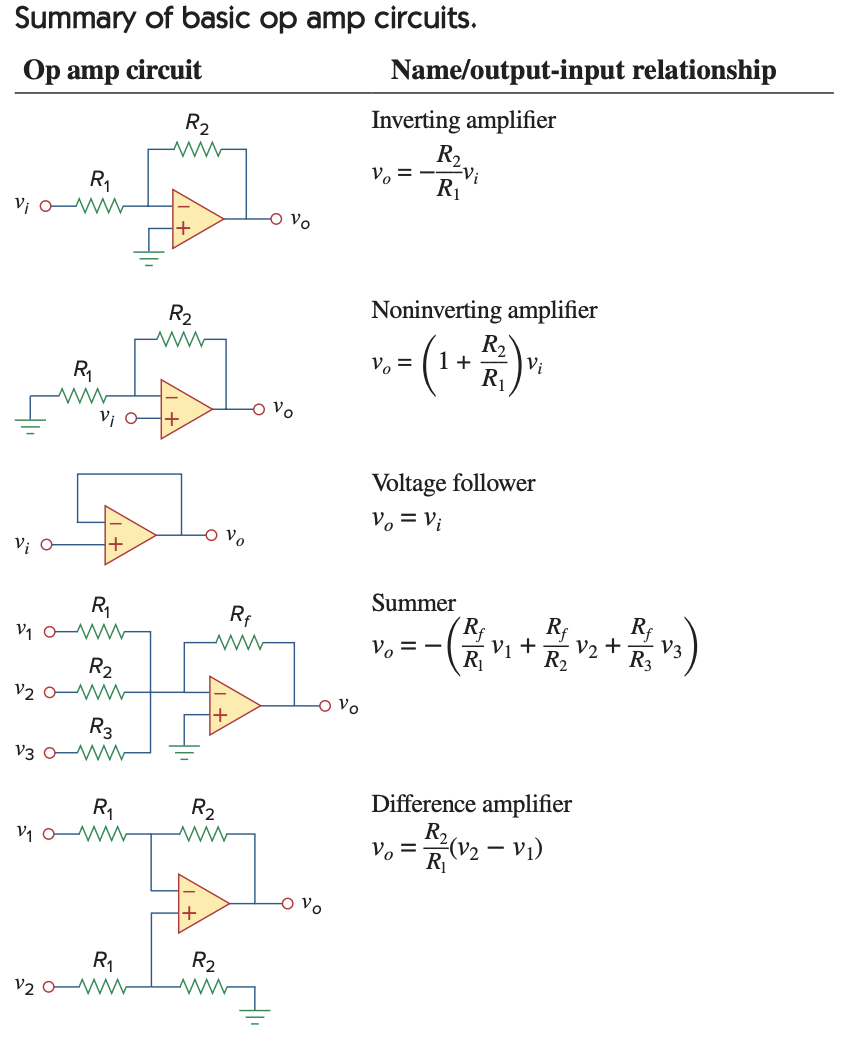
\includegraphics[width=0.9\linewidth]{AppendixItems/OpAmps.png}
    \centering
    \caption{Common Op-Amp Circuits}
\end{figure}
\end{document}
